 
 % Uses:
 %		SETTINGS.TEX	contains the settings for this document
 %		COMMANDS.TEX	contains commands which can be used while writing
 %		INFO.TEX			contains the author, title and so on for the cover
 %		COVER.TEX			formats the front cover of the document
 %		ABSTRACT.TEX	contains the abstract to be included (if needed)
 %		BIB.BIB				containt the BibTeX entries for the document
 
\documentclass[11pt,a4paper,bibtotoc,idxtotoc,headsepline,footsepline,footexclude,BCOR12mm,DIV13]{scrbook}

% KOMA-Optionen:
%  bibtotoc: include bibliography in table of contents
%  idxtotoc: include index in table of contents
%  headsepline: use horizontalline under heading
%  BCOR: binding correcion (Bindungskorrektur) (e.g.: BCOR5mm)
%  DIV: Number of sheet sections (used for layout) (e.g.: DIV12) 

% include title and author information for the cover
% Set here the title, authors and other stuff to be used for the cover
% This file is used by MAIN.TEX

% set title, authors and stuff for the cover
\def\doctype{Interdisciplinary Project in Finance and Informatics}
\def\title{Leads and Lags of Corporate Bonds and Stocks}
\def\titleGer{Leads und Lags von Unternehmensanleihen und Aktien}
\def\author{Alex Kulikov}
\def\date{March 31, 2021}

% text to appear in the footer
\def\footertext{}

% include settings
% Included by MAIN.TEX
% Defines the settings for the CAMP report document

\renewcommand{\sectfont}{\normalfont \bfseries}        % Schriftart der Kopfzeile

% manipulate footer
\usepackage{scrpage2}
\pagestyle{scrheadings}
\ifoot[\footertext]{\footertext} % \footertext set in INFO.TEX
%\setkomafont{pagehead}{\normalfont\rmfamily}
\setkomafont{pagenumber}{\normalfont\rmfamily}

%% allow sophisticated control structures
\usepackage{ifthen}

% use Palatino as default font
\usepackage{palatino}

% enable special PostScript fonts
\usepackage{pifont}

% make thumbnails
\usepackage{thumbpdf}

%to use the subfigures
\usepackage{subfigure}


\usepackage{colortbl}


%% show program code\ldots
%\usepackage{verbatim}
%\usepackage{program}
\usepackage{minted}
\usepackage{listings}

\usepackage{caption}

% writing pseudo-code
\usepackage{algorithm}
%\usepackage{algorithmic}
\usepackage[noend]{algpseudocode}% http://ctan.org/pkg/algorithmicx
%\usepackage[linesnumbered,ruled]{algorithm2e}

%% enable TUM symbols on title page
\usepackage{styles/tumlogo}


\usepackage{multirow}

%% use colors
\usepackage{color}

%% make fancy math
\usepackage{amsmath}
\usepackage{amsfonts}
\usepackage{amssymb}
\usepackage{textcomp}
\usepackage{yhmath} % f�r die adots 
%% mark text as preliminary
%\usepackage[draft,german,scrtime]{prelim2e}

%% create an index
\usepackage{makeidx}

% for the program environment
\usepackage{float}

%% load german babel package for german abstract
%\usepackage[german,american]{babel}
\usepackage[german,english]{babel}
\selectlanguage{english}

% use german characters as well
\usepackage[latin1]{inputenc}       % allow Latin1 characters

% use initals dropped caps - doesn't work with PDF
\usepackage{styles/dropping}


\usepackage{styles/shortoverview}
%----------------------------------------------------
%      Graphics and Hyperlinks
%----------------------------------------------------

%% check for pdfTeX
\ifx\pdftexversion\undefined
 %% use PostScript graphics
 \usepackage[dvips]{graphicx}
 \DeclareGraphicsExtensions{.eps,.epsi}
 \graphicspath{{figures/}{figures/review}} 
 %% allow rotations
 \usepackage{rotating}
 %% mark pages as draft copies
 %\usepackage[english,all,light]{draftcopy}
 %% use hypertex version of hyperref
 \usepackage[hypertex,hyperindex=false,colorlinks=false]{hyperref}
\else %% reduce output size \pdfcompresslevel=9
 %% declare pdfinfo
 %\pdfinfo { 
 %  /Title (my title) 
 %  /Creator (pdfLaTeX) 
 %  /Author (my name) 
 %  /Subject (my subject	) 
 %  /Keywords (my keywords)
 %}
 %% use pdf or jpg graphics
 \usepackage[pdftex]{graphicx}
 \DeclareGraphicsExtensions{.jpg,.JPG,.png,.pdf,.eps}
 \graphicspath{{figures/}} 
 
 %% Load float package, for enabling floating extensions
 \usepackage{float}
 
 %% allow rotations
 \usepackage{rotating}
 %% use pdftex version of hyperref
 \usepackage[pdftex,colorlinks=true,linkcolor=black,citecolor=black,%
 anchorcolor=black,urlcolor=black,bookmarks=true,%
 bookmarksopen=true,bookmarksopenlevel=0,plainpages=false%
 bookmarksnumbered=true,hyperindex=false,pdfstartview=%
 ]{hyperref}
%
%\usepackage[pdftex,colorlinks=false,linkcolor=red,citecolor=red,%
% anchorcolor=red,urlcolor=red,bookmarks=true,%
% bookmarksopen=true,bookmarksopenlevel=0,plainpages=false%
% bookmarksnumbered=true,hyperindex=false,pdfstartview=%
% ]{hyperref}
\fi




%% Fancy chapters
%\usepackage[Lenny]{fncychap}
%\usepackage[Glenn]{fncychap}
%\usepackage[Bjarne]{fncychap}

%\usepackage[avantgarde]{quotchap}

% set the bibliography style
%\bibliographystyle{styles/bauermaNum}
%\bibliographystyle{alpha}
\bibliographystyle{plain}

% include commands
% Commands to be used within the TUM report document
% Included by MAIN.TEX
% Please include your own cool commands here. 
% Be only sure to comment it sufficiently so others can use it.

%-------------------------------------------------------------
%                      Own Commands
%-------------------------------------------------------------


%-------------------------------------------------------------
% math stuff -------------------------------------------------

% nice R, N, C
\newcommand{\nat}{\mathbb{N}}
\newcommand{\real}{\mathbb{R}}
\newcommand{\compl}{\mathbb{C}}



% norm
\newcommand{\norm}[1]{\left\| #1 \right\|}

% un demi
\newcommand{\half}{\frac{1}{2}}

% parantheses
\newcommand{\parenth}[1]{ \left( #1 \right) }
\newcommand{\bracket}[1]{ \left[ #1 \right] }
\newcommand{\accolade}[1]{ \left\{ #1 \right\} }
%\newcommand{\angle}[1]{ \left\langle  #1 \right\rangle }

% partial derivative: %#1 function, #2 which variable
% simple / single line version
\newcommand{\pardevS}[2]{ \delta_{#1} f(#2) }
% fraction version
\newcommand{\pardevF}[2]{ \frac{\partial #1}{\partial #2} }

% render vectors: 3 and 4 dimensional
\newcommand{\veciii}[3]{\left[ \begin{array}[h]{c} #1 \\ #2 \\ #3	\end{array} \right]}
\newcommand{\veciv}[4]{\left[ \begin{array}[h]{c} #1 \\ #2 \\ #3 \\ #4	\end{array} \right]}

% render matrices: 3  dimensional (arguments in row first order)
\newcommand{\matiii}[9]{\left[ \begin{array}[h]{ccc} #1 & #2 & #3 \\ #4 & #5 & #6 \\ #7 & #8 & #9	\end{array} \right]}
%DOESN'T WORK,DON'T KNOW WHY \newcommand{\mativ}[16]{\left[ \begin{array}[h]{cccc} #1 & #2 & #3 & #4 \\ #5 & #6 & #7 & #8 \\ #9 & #10 & #11 & #12 \\ #13 & #14 & #15 & #16 \end{array} \right]}


%-------------------------------------------------------------
%-------------------------------------------------------------


%-------------------------------------------------------------
% some abreviations ------------------------------------------
\newcommand{\Reg}{$^{\textregistered}$}
\newcommand{\reg}{$^{\textregistered}$ }
\newcommand{\Tm}{\texttrademark}
\newcommand{\tm}{\texttrademark~}
\newcommand {\bsl} {$\backslash$}

%-------------------------------------------------------------
%-------------------------------------------------------------


%-------------------------------------------------------------
% formating --------------------------------------------------

% Theorem & Co environments and counters
\newtheorem{theorem}{Theorem}[chapter]
\newtheorem{lemma}[theorem]{Lemma}
\newtheorem{corollary}[theorem]{Corollary}
\newtheorem{remark}[theorem]{Remark}
\newtheorem{definition}[theorem]{Definition}
\newtheorem{equat}[theorem]{Equation}
\newtheorem{example}[theorem]{Example}
%\newtheorem{algorithm}[theorem]{Algorithm}

% inserting figures
\newcommand{\insertfigure}[4]{ % Filename, Caption, Label, Width percent of textwidth
	\begin{figure}[htbp]
		\begin{center}
			\includegraphics[width=#4\textwidth]{#1}
		\end{center}
		\vspace{-0.4cm}
		\caption{#2}
		\label{#3}
	\end{figure}
}




% referecing figures

\newcommand{\refFigure}[1]{ %label
	figure \ref{#1}
}
\newcommand{\refChapter}[1]{ %label
	chapter \ref{#1}
}

\newcommand{\refSection}[1]{ %label
	section \ref{#1}
}

\newcommand{\refParagraph}[1]{ %label
	paragraph \ref{#1}
}

\newcommand{\refEquation}[1]{ %label
	equation \ref{#1}
}

\newcommand{\refTable}[1]{ %label
	table \ref{#1}
}




\newcommand{\rigidTransform}[2]
{
	${}^{#2}\!\mathbf{H}_{#1}$
}

%code, in typewriter
\newcommand{\code}[1]
 {\texttt{#1}}

% comment that appears on the border - very practical !!!
\newcommand{\comment}[1]{\marginpar{\raggedright \noindent \footnotesize {\sl #1} }}

% page clearing
\newcommand{\clearemptydoublepage}{%
  \ifthenelse{\boolean{@twoside}}{\newpage{\pagestyle{empty}\cleardoublepage}}%
  {\clearpage}}


%-------------------------------------------------------------
%-------------------------------------------------------------


\newcommand{\etAl}{\emph{et al.}\mbox{ }}

\makeglossary

\begin{document}
	
	% New definitions
	\algnewcommand\algorithmicswitch{\textbf{switch}}
	\algnewcommand\algorithmiccase{\textbf{case}}
	\algnewcommand\algorithmicassert{\texttt{assert}}
	\algnewcommand\Assert[1]{\State \algorithmicassert(#1)}%
	% switch case
	\algdef{SE}[SWITCH]{Switch}{EndSwitch}[1]{\algorithmicswitch\ #1\ \algorithmicdo}{\algorithmicend\ \algorithmicswitch}%
	\algdef{SE}[CASE]{Case}{EndCase}[1]{\algorithmiccase\ #1}{\algorithmicend\ \algorithmiccase}%
	\algtext*{EndSwitch}%
	\algtext*{EndCase}%
	% parallel_for
	\algnewcommand\algorithmicpfor{\textbf{parallel\_for}}
	\algdef{SE}[PFOR]{PFor}{EndPFor}[1]{\algorithmicpfor\ #1\ \algorithmicdo}{\algorithmicend\ \algorithmicpfor}%
	\algtext*{EndPFor}%
	

	\frontmatter		
		%% The front cover for the TUM report document.
% Included by MAIN.TEX


%--------------------------------------------------
% The Front Cover
%--------------------------------------------------

% The front cover for the TUM document.
% Included by MAIN.TEX


%--------------------------------------------------
% The Front Cover
%--------------------------------------------------

% correct BCOR - undo at the end !!!
\def\bcorcor{0.15cm}
\addtolength{\hoffset}{\bcorcor}

\thispagestyle{empty}

 \vspace{4cm}
\begin{center}
	       \oTUM{4cm}
	   
	   \vspace{5mm}     
	   \huge DEPARTMENT OF INFORMATICS\\ 
	   \vspace{0.5cm}
	 \large TECHNICAL UNIVERSITY OF MUNICH\\
    \vspace{1mm}
        
	\end{center}
		

\vspace{15mm}
\begin{center}

   {\Large \doctype}

  \vspace{20mm}
  
  {\huge\bf \title}\\%[3ex]
  
  
  \vspace{15mm}
  
  
  {\LARGE  \author}
  
  \vspace{10mm}
  
  \begin{figure}[h!]
  \centering
   
\includegraphics[width=4cm]{styles/informat.png}
  \end{figure}
  
  \end{center}		
		%\clearemptydoublepage	
		%% The titlepage for the CAMP report document.
% Included by MAIN.TEX


%--------------------------------------------------
% The title page
%--------------------------------------------------

% correct BCOR - undo at the end !!!
\def\bcorcor{0.15cm}
\addtolength{\hoffset}{\bcorcor}

\thispagestyle{empty}

 \vspace{10mm}
\begin{center}
	       \oTUM{4cm}
	   
	   \vspace{5mm}     
	   \huge DEPARTMENT OF FINANCE\\ 
	   \vspace{0.5cm}
	 \large TECHNICAL UNIVERSITY OF MUNICH\\
        
	\end{center}
		

\vspace{10mm}
\begin{center}

   {\Large \doctype}

  \vspace{10mm}
  
  {\LARGE \title}\\
  
  
  \vspace{10mm}
  
  
  {\LARGE  \titleGer}\\
  
  
  \vspace{10mm}

    %\hfill
    \begin{tabular}{ll}
	   \Large Author:     & \Large \author \\[2mm]
	   \Large Supervisor:    & \Large Prof. Dr. Sebastian M\"{u}ller \\[2mm]				
	   \Large Advisor:	& \Large Zihan Gong \\[2mm]
	   \Large Date:       & \Large March 31, 2021
	 \end{tabular}
	 
	 \vspace{5mm}
	 
	 \begin{figure}[h!]
  \centering
   
\includegraphics[width=4cm]{styles/informat.png}
  \end{figure}
   

\end{center}

% undo BCOR correction
\addtolength{\hoffset}{\bcorcor}	
		%\input{components/cover_maschmeyer}	
		%\clearemptydoublepage			
		% The titlepage for the CAMP report document.
% Included by MAIN.TEX


%--------------------------------------------------
% The title page
%--------------------------------------------------

% correct BCOR - undo at the end !!!
\def\bcorcor{0.15cm}
\addtolength{\hoffset}{\bcorcor}

\thispagestyle{empty}

 \vspace{10mm}
\begin{center}
	       \oTUM{4cm}
	   
	   \vspace{5mm}     
	   \huge DEPARTMENT OF FINANCE\\ 
	   \vspace{0.5cm}
	 \large TECHNICAL UNIVERSITY OF MUNICH\\
        
	\end{center}
		

\vspace{10mm}
\begin{center}

   {\Large \doctype}

  \vspace{10mm}
  
  {\LARGE \title}\\
  
  
  \vspace{10mm}
  
  
  {\LARGE  \titleGer}\\
  
  
  \vspace{10mm}

    %\hfill
    \begin{tabular}{ll}
	   \Large Author:     & \Large \author \\[2mm]
	   \Large Supervisor:    & \Large Prof. Dr. Sebastian M\"{u}ller \\[2mm]				
	   \Large Advisor:	& \Large Zihan Gong \\[2mm]
	   \Large Date:       & \Large March 31, 2021
	 \end{tabular}
	 
	 \vspace{5mm}
	 
	 \begin{figure}[h!]
  \centering
   
\includegraphics[width=4cm]{styles/informat.png}
  \end{figure}
   

\end{center}

% undo BCOR correction
\addtolength{\hoffset}{\bcorcor}	
		%%\thispagestyle{empty}
\selectlanguage{english}
	%\vspace*{0.8\textheight}
	%\noindent
	I confirm that this documentation as part of my interdisciplinary project is my own work and I have documented all sources and material used.
	
	%\vspace{15mm}
	%\noindent
	%Munich, \today \hspace{5cm} \author
\selectlanguage{english}	
		%\clearemptydoublepage
\phantomsection
\addcontentsline{toc}{chapter}{Acknowledgements}	


%\chapter*{Acknowledgements}

\vspace*{2cm}

\begin{center}
{\Large \bf Acknowledgments}
\end{center}

\vspace{1cm}




	
		% Abstract for the TUM report document
% Included by MAIN.TEX

\phantomsection
\addcontentsline{toc}{chapter}{Abstract}	

\vspace*{2cm}
\begin{center}
{\Large \bf Abstract}
\end{center}
\vspace{1cm}

In the scope of an Interdisciplinary Project at the Technical University of Munich, an international, extendable corporate bonds database had to be built up from scratch for further empirical research. For this purpose, an automatic extraction tool for financial securities data has been developed on top of the interface provided by the Refinitiv Datastream financial database. The required static and time series corporate bond data -- consisting of over 60.000 bonds -- has been downloaded, cleaned, and prepared for further research. Additionally, a matching algorithm has been developed to join corporate bond and stock data with each other based on their issuing company. The algorithm utilizes fuzzy string matching based on company name as well as key-based matching based on the CUSIP-9 parameter, and has shown a matching ratio of around 45\% without a globally unique company identifier. Further, the distribution of corporate bond returns has been found in-line with expectations, which served as a sanity check for the downloaded data. Finally, correlation and regression analyses have shown stock data to be more efficient in incorporating new information than corporate bond data based on a 1-month lead. 

		%% German abstract for the CAMP report document
% Included by MAIN.TEX


\clearemptydoublepage






\vspace*{2cm}
\begin{center}
{\Large \bf Zusammenfassung}
\end{center}
\vspace{1cm}

Die vorliegende Arbeit befasst sich mit der Anpassung und Parallelisierung effizienter Skyline Algorithmen f�r moderne Hauptspeicher-Datenbanksysteme. Au�erdem richtet sie den ART Baum f�r kategorische Skyline Berechnung ein. 

Um Datenbank-Anfragen schneller bearbeiten zu k�nnen, werden einige der bekannten Skyline Algorithmen so angepasst, dass sie als Baustein direkt in eine Hauptspeicher-Datenbank aufgenommen werden k�nnen. Daraufhin werden moderne Parallelisierungstechniken vorgestellt und auf die Skyline Algorithmen angewendet. Die gemessenen Performanzergebnisse bezeugen, dass die vorgeschlagenen Parallelisierungsans�tze die Laufzeit der Algorithmen in parallelisierter Umgebung verbessern konnten. 

Dar�ber hinaus wurde der ART Baum dazu verwendet, den neuartigen Algorithmus SARTS zu entwerfen. Der Algorithmus eignet sich besonders gut zur progressiven Berechnung der Skyline in Online-Umgebungen. Im Rahmen der durchgef�hrten Tests zeigt der Algorithmus sehr solide Laufzeiten auch bei gr��eren Tupelmengen und verbraucht dabei bis zu 20-mal weniger Speicher als sein direkter Vorg�nger ST-S. %Letzteres verdankt er dem effizienten Speicherumgang des ART Baums. 

%Mit steigender Nachfrage nach interaktiven Services im Internet w�chst auch der Bedarf nach effizienten Algorithmen, welche sich mit der Verarbeitung der entstehenden Datenmengen befassen. Eine der heutzutage immer h�ufiger eingesetzten Methoden zur Filterung der Datenbasis ist die Berechnung der Skyline einer Menge von Tupeln. Zu der Skyline geh�ren diejenigen Tupel, welche interessant f�r den Anfragesteller sind. Ein Tupel gilt als interessant, sofern es von keinem anderen Tupel aus der Datenmenge dominiert wird. 



		\tableofcontents
		%\clearemptydoublepage

\phantomsection
%\addcontentsline{toc}{chapter}{Outline of the Thesis}

%\begin{center}
%	\huge{Outline of the Thesis}
%\end{center}
%
%
%
%
%%--------------------------------------------------------------------
%\section*{Part I: Introduction and Theory}
%
%\noindent {\scshape Chapter 1: Introduction}  \vspace{1mm}
%
%\noindent  This chapter presents an overview of the thesis and it purpose. Furthermore, it will discuss the sense of life in a very general approach.  \\
%
%\noindent {\scshape Chapter 2: Theory}  \vspace{1mm}
%
%\noindent  No thesis without theory.   \\
%
%%--------------------------------------------------------------------
%\section*{Part II: The Real Work}
%
%\noindent {\scshape Chapter 3: Overview}  \vspace{1mm}
%
%\noindent  This chapter presents the requirements for the process.

	\mainmatter	
%		\part[Introduction and Theory]{Introduction and Theory}
%		\label{part:introAndBackgroundTheory}

		\chapter{Introduction} \label{chapter:Introduction}
In the scope of an Interdisciplinary Project (\textit{IDP} in the following) at the Technical University of Munich, the lead and lag relationship between corporate bond and stock returns has to be analyzed. With the needed stock data already provided, the first step of the IDP is to develop a tool which would be able to automatically extract static and time series data from the Thomson Reuters Datastream financial database. In the second step of the IDP, the extracted bond data has to be cleaned and prepared for further analysis by various transformation techniques. Additionally, a matching approach to join the stock and bond datasets by issuing company needs to be developed. In the third and final step of the IDP, the resulting bond-stock database has to be checked for any sort of lead and/or lag relationships within bond and stock return pairs. 

The extracted corporate bond data, both static and time series, has a wide array of applications, ranging from descriptive historical applications to predictive models, and will thus be of significant value for future financial research. In order to make use of the most recent market trends and developments, the acquired bond database, as well as the existing stock information, should be extendable, such that recent data can be accumulated in a continuous manner. This is where the tool for automated data extraction from Refinitiv Datastream comes into play. It has to provide capabilities to download financial securities data in a convenient and seamless manner, as far as technology allows. Since corporate bonds and their qualities as an investment instrument are often compared to equities \cite{asset-management}, it only makes sense to additionally develop an efficient approach to analyze the two asset classes "side-by-side". At this point, a suitable matching mechanism to join bond and equity data by their issuing company is of paramount importance, and can be used in many different analysis scenarios. At the end of any financial analysis, researchers are always interested in the insights into the functioning of financial markets and the optimal investment thesis which arises therefrom. Analyzing the lead and lag relationship of corporate stocks and bonds can provide such an investment thesis based on the efficiency with which the two asset classes incorporate new information in their pricing \cite{lead-lag-source}. From a practical perspective, if I, as an investor, knew that today's stock returns predict bond returns in the next month, I could allocate my assets accordingly to gain a higher-than-usual profit from my investment. While the constraints and influence of market equilibrium conditions on such an investment strategy could be analyzed separately \cite{asset-management}, the gain of such knowledge is undoubtedly of significant academical and practical importance. 



		\chapter{Skyline Computation} \label{chapter:skyline-computation}
Various algorithms have been developed to compute the skyline of a given set of tuples. To date, no multipurpose skyline algorithm exists that would perform equally well in every environment and under any circumstances. Therefore, a number of algorithms have recently emerged that are each tailored to some very specific range of skyline problems. In this chapter, some of the most relevant up-to-date skyline algorithms are briefly introduced and the necessary theoretical foundation to the term skyline is given. 

\section{The Skyline Operator} \label{section:skyline-operator}
From a theoretical point of view, computing the skyline of a set of tuples corresponds to the mathematical problem of finding the maxima of a set of vectors~\cite{kung}. While the problem has been extensively described and analyzed by Kung et al. as early as in 1975~\cite{kung}, the term skyline in the context of databases was first introduced by D. Kossmann et al. in 2001~\cite{kossmann}, along with the first efficient skyline algorithms. 

The skyline of a set of tuples is defined as those tuples that are not dominated by any other tuple in the set. A tuple $p$ dominates a tuple $q$ if $p$ is not worse than $q$ in every given dimension and is better than $q$ in at least one dimension. Or, equally, 
\begin{equation}
p \succ q := \nexists i \in N^{+}_{0} . p[A_{i}] > q[A_{i}] \wedge \exists j \in N^{+}_{0} . p[A_{j}] < q[A_{j}]. 
\end{equation}
The definition assumes that the tuple attributes in each dimension have to be minimized. If they have to be maximized instead, then the $>$ and $<$ signs have to be flipped respectively. The notation $p[A_{i}]$ (resp. $q[A_{i}]$) stands for $p$'s (resp. $q$'s) $i$-th attribute value. 

%The process of computing the skyline of a range of tuples is visualized in Fig.~\ref{fig:skyline-example} for the apartment example. 



% maybe add that skyline operation is related to top-k queries etc. 

To integrate the operation of skyline computation into a database system was first proposed by Kossmann et al.~\cite{kossmann} in 2001. The researchers suggested a skyline extension to SQL that would filter out the tuples from the underlying database that are not worse than any other tuple. The SQL syntax proposed to be incorporated into the structure of a query would be similar to: 
\begin{minted}{sql}
SELECT ... FROM ... WHERE ...
GROUP BY ... HAVING ...
SKYLINE OF [DISTINCT] d1 [MIN | MAX], ... , dn [MIN | MAX]
ORDER BY ...
\end{minted}
Herein, $d_{1}$, ... , $d_{n}$ are the dimensions of the skyline. The annotations $MIN$ and $MAX$ specify for each dimension whether it has to be minimized or maximized. 
The authors argue that implementing the functionality of the skyline operator on top of the database is both costly and inefficient, and thus propose the new operator to be integrated directly into the database. 

\section{Database Context} \label{section:database-context}
The implementation of the skyline operator inside a database system is influenced by several, sometimes contradictory, criteria. These are, among others, the type of the database, its estimated size, the prevalent data types used, the requirements regarding time and resource usage, as well as the particular use cases in mind at the time of database design. 

% existence of an index, possibility of parallelization, cpu processing power, available main memory, communication with disc required or not 
One of the most common optimization approaches is to reduce the number of needed dominance checks, in order to compute the skyline with a lesser number of comparisons. This way, the CPU cost of the skyline operation can be significantly reduced. Therefore, this optimization technique is most sensible for database systems with generally limited computation resources. One of the algorithms taking this path of optimization is the ST-S algorithm \cite{rahman}, which will be discussed later in greater detail. 
The main drawback of such algorithms is generally higher memory usage, as the number of dominance checks is most easily reduced by using an extra data structure to ''sift'' the tuples through it. In most cases, this is some specially fitted form of tree which enables a significant reduction in tuple comparisons. This is why only database systems with a sufficient amount of main memory available at runtime are eligible for this type of optimization. For this reason, in-memory databases seem optimally fitted for such algorithms. 

Another criterion to account for is the estimated size of the original dataset. While some algorithms show excellent running times on low numbers of tuples, their runtime grows exponentially with the rising size of the input. Other algorithms, however, are best suited for very large datasets, usually by enabling various parallelization approaches. Large multicore database systems, specially optimized for computation-intensive OLAP queries are the best prerequisite for such algorithms. Some of the approaches are based on the well-known divide-and-conquer principle to achieve this goal. 

For database systems with frequent background storage access, a different optimization technique has been developed. In order to conduct the entire computation process within the (often limited) main memory, the tuples for the computation are always loaded block-wise, and the number of I/O accesses to the background storage is thus reduced. Block-Nested-Loops~\cite{kossmann} is one the most basic, but nonetheless efficient algorithms for this purpose. 

Depending on the data type of the attribute values stored in the tuples, some algorithms might prove not eligible for the particular scenario at all. This is for instance the case with tree-based algorithms where each attribute can only assume categorical values. The reason for this is that each node can maximally have as many child nodes as there are allowed attribute values. While this is usually not a problem for some bounded number of integer values, there are simply too many possible double values between any two range boundaries to create a new child node for each of them. 

%In addition to that, whenever an index structure exists on the tuples of the database, it can also be used to improve the performance of the skyline operation. Some of the algorithms taking this path will be further discussed in related work (section~\ref{section:related-work}). %are NN~\cite{nn} and BBS~\cite{bbs}, both based on Nearest-Neighbor-Search.

In the following and throughout this paper, a hybrid main-memory database system, such as HyPer~\cite{hyper}, is assumed as the context of this work. It combines the advantages of both OLTP and OLAP databases in one, and thus enables most of the optimization techniques mentioned above. While optimization approaches such as bulk-loading of the tuples into main memory are no longer required, improvements like tree-based dominance tests and also parallelization become possible. 

\section{Related Work} \label{section:related-work}
While a lot of work has been done developing high-performing algorithms for skyline computation, many aspects of the field are still not entirely covered. Such aspects include memory efficiency for progressive skyline algorithms, as well as parallelization of originally sequential approaches. The following section gives an overview of some of the most prominent skyline algorithms to date. 

\subsection{Naive-Nested-Loops Algorithm} \label{subsection:naive-nested-loops}
Arguably the simplest existing skyline algorithm is Naive-Nested-Loops. As mentioned by Kossmann et al, ``[t]his is essentially what happens if a Skyline query is implemented on top of a database system''\cite{kossmann}. 

The main idea behind the algorithm is to compare each tuple of the dataset with every other tuple. This is accomplished by creating two loops, one of them nested in the other, and for each tuple to traverse the entire dataset from beginning to end, in order to check whether the tuple is dominated by any other. If it is not dominated, then it is added to the resulting skyline. While Naive-Nested-Loops is very versatile and can be applied to almost every given dataset, it tends to perform badly in comparison to some of the newer algorithms. A pseudo-code notation of the algorithm is shown in Algorithm \ref{alg:nnl}. 

% pseudo-code Naive Nested-Loops
\begin{algorithm}[h]
	\caption{Naive Nested-Loops Algorithm} \label{alg:nnl}
	\begin{algorithmic}[1] 
		\State \textbf{Input :} Tuple List $T$
		\State \textbf{Output :} Skyline $skyline$
		\For {each tuple $t~\in~T$}
			\State $is\_not\_dominated \gets $True
			\For {each tuple $d~\in~T\backslash\{t\}$}
				\If {dominates($d$, $t$)}
					\State $is\_not\_dominated \gets $False
					\State Exit inner loop
				\EndIf
			\EndFor
			\If {$is\_not\_dominated$}
				\State Add $t$ to $skyline$
			\EndIf
		\EndFor
	\end{algorithmic}
\end{algorithm}

\subsection{Block-Nested-Loops Algorithm} \label{subsection:bnl}
One of the most basic skyline algorithms, and yet fairly efficient, is the Block-Nested-Loops~\cite{kossmann} algorithm (in the following BNL). It takes the concept of Naive-Nested-Loops and extends it by making sure that incomparable tuples are kept in a persisting \textit{window} in main memory. The main idea behind this is to reduce the number of necessary I/O operations when working with traditional DBMS, as disc storage has significantly longer access times than main memory~\cite{book-kemper}. 

Whenever a new tuple is inserted into the window, it is iteratively compared to all the other tuples that already find themselves in the window. At this point, one of the following happens: 
\begin{itemize}
	\item If the new tuple is dominated by some other tuple in the window, then it is eliminated and is no longer considered for the skyline. 
	\item If the new tuple dominates one or more of the other tuples in the window, then these tuples are eliminated from the window and are no longer considered for the skyline. The new tuple gets inserted into the window as a new skyline candidate. 
	\item If the new tuple is incomparable with all the other tuples in the window and there is enough space left in it, then it gets inserted. If there is not enough space in the window, then the new tuple is written to the temporary file on disc and will be considered again for further iterations of the algorithm. The last step with the temporary file is not necessary if a main memory database is used, because in this case all the incomparable tuples fit into the window. 
\end{itemize}
All the tuples that are left in the window at the end of each iteration and that have been compared to all the tuples in the temporary file, can be output as part of the skyline. For the original algorithm, the researchers propose to accomplish this by assigning \textit{timestamps} to the tuples~\cite{kossmann}. This way, one can determine in which order the tuples have originally been read in. The tuples that have been output before the algorithm terminates are part of the skyline. At this point, all the other tuples from the original dataset have been eliminated. 

The pseudo-code of the in-memory version of the BNL algorithm, which is used in this work, is shown in Algorithm \ref{alg:bnl}. It only needs one iteration based on the original set of tuples, and does not require a temporary file because all skyline tuples fit into main memory. 

% pseudo-code Block-Nested-Loops
\begin{algorithm}[h]
	\caption{Block-Nested-Loops Algorithm (in-memory)} \label{alg:bnl}
	\begin{algorithmic}[1] 
		\State \textbf{Input :} Tuple List $T$, Window $window$
		\State \textbf{Output :} Skyline $skyline$
		\State $t_{0} \gets $ first element of $T$
		\State Add $t_{0}$ to $window$
		\For {each tuple $t~\in~T\backslash\{t_{0}\}$}
			\State Add $t$ to $window$
			\For {each tuple $d~\in~window\backslash\{t\}$}
				\If {dominates($t$, $d$)}
					\State Eliminate $d$ from $window$
				\EndIf
				\If {dominates($d$, $t$)}
					\State Eliminate $t$ from $window$
					\State Exit inner loop 
				\EndIf
			\EndFor
		\EndFor
		\State Return $window$ as $skyline$
	\end{algorithmic}
\end{algorithm}

%The best-case complexity of the algorithm is in the magnitude of $O(n)$ and can be achieved when the entire skyline fits into the window~\cite{kossmann}. This way, only one run of the algorithm is necessary, no temporary file is needed and the entire resulting skyline finds itself in the window right after the first iteration. The worst-case complexity of BNL is $O(n^{2})$~\cite{kossmann}. It is exactly the same as for the Naive-Nested-Loops algorithm and occurs when each tuple has to be compared to every other tuple in the underlying dataset. 
BNL cannot output any of its results before the entire skyline has been computed~\cite{survey}. This is because even the last of the remaining tuples can eliminate some of the candidate tuples that find themselves in the window. 
Moreover, while the I/O behavior of this algorithm is significantly superior to that of Naive-Nested-Loops, this advantage gets lost when working with an in-memory database system. The advantage of not having to compare every tuple with every other tuple, however, is still a major improvement. 
A more detailed description of the BNL algorithm can be found in the original paper \cite{kossmann}. 

\subsection{Divide-and-Conquer Algorithm} \label{subsection:dnc}
The Divide-and-Conquer algorithm \cite{kossmann, kung} follows the well-known divide-and-conquer principle, when the original problem is first divided into smaller sub-problems, in order to minimize the workload to solve each of them individually. The algorithm recursively partitions the original dataset into smaller datasets, until each of the subsets only consists of one tuple. For the partitioning, the median $m_{d}$ of the current dataset is determined for one of the dimensions, let us call it $d$. This paper assumes the version of the algorithm in which $d$ is initialized as the last of the given dimensions. The first partition $P_{1}$ is then filled with tuples that have lesser attribute values in this dimension than the median. The second partition $P_{2}$ is filled with tuples that have greater or equal attribute values in this dimension than the median. In order to determine the median, it is sometimes sensible to presort the tuples of the original dataset according to dimension $d$. The partitioning process is visualized in Fig.~\ref{fig:dnc-partitioning}. 

\begin{figure}[h]
\centering
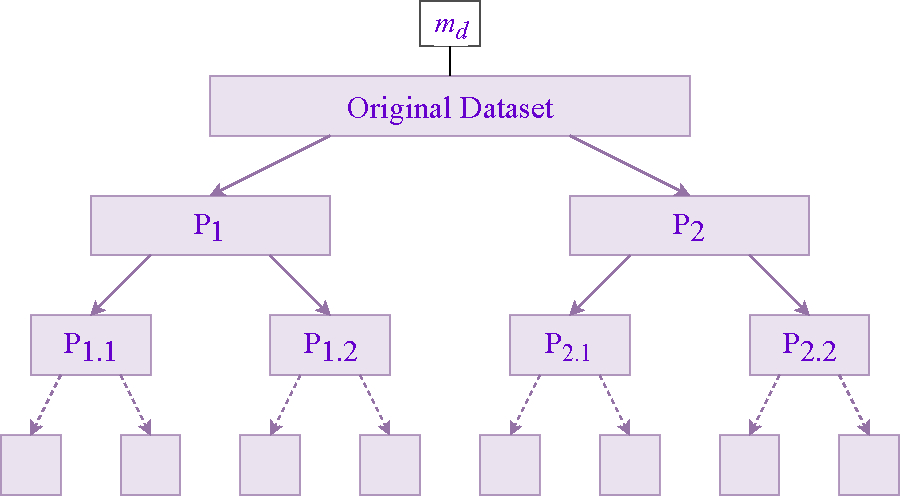
\includegraphics[width=0.7\linewidth]{figures/dnc-partitioning}
\caption{DNC Partitioning Process}
\label{fig:dnc-partitioning}
\end{figure}

When the recursive partitioning is completed, the resulting subsets get merged starting with the smallest ones. Whenever two partitions $P_{1}$ and $P_{2}$ are merged, the tuples in $P_{2}$ that are dominated by any tuple in $P_{1}$ are eliminated. The tuples in $P_{1}$ cannot be dominated by tuples from $P_{2}$, because they are \`{a}-priori better than the tuples in $P_{2}$ in at least one dimension, which is $d$. This is due to the division of the original dataset according to the median $m_{d}$. Hence, only incomparable tuples are left when the merging is complete. 
The merge process is illustrated in Fig.~\ref{fig:dnc-merging}. 

\begin{figure}[h]
\centering
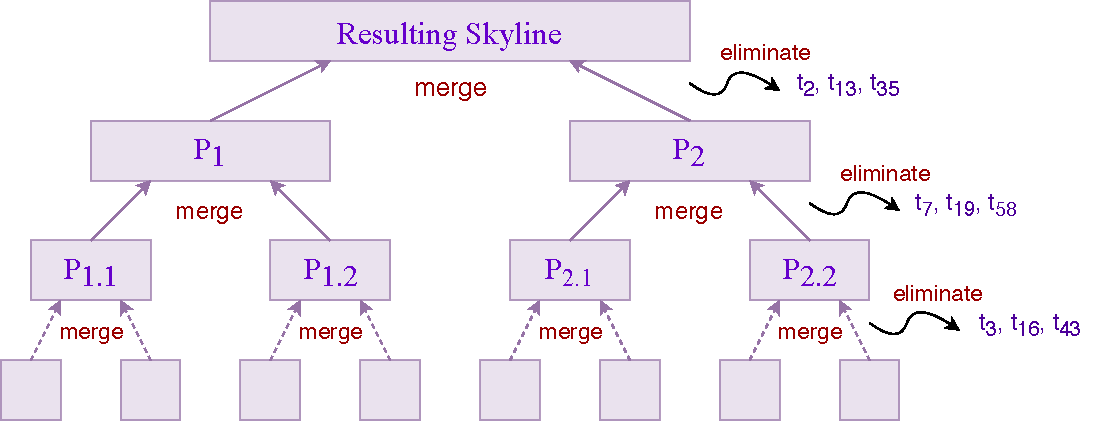
\includegraphics[width=0.9\linewidth]{figures/dnc-merging}
\caption{DNC Merging Process}
\label{fig:dnc-merging}
\end{figure}

Kossmann et al. \cite{kossmann} suggest to further improve the merging process by once again applying the divide-and-conquer principle. For this purpose, each of the two partitions $P_{1}$ and $P_{2}$ gets partitioned again; this time according to a different dimension ($d-1$ for instance). $P_{1}$ and $P_{2}$ are now split into $P_{1.1}$ and $P_{1.2}$, and $P_{2.1}$ and $P_{2.2}$, respectively. This has the advantage that not all tuples in $P_{1}$ and $P_{2}$ have to be compared to each other. Instead, now only the tuples in $P_{1.1}$ and $P_{2.1}$, in $P_{1.2}$ and $P_{2.2}$, and in $P_{1.1}$ and $P_{2.2}$ need to be compared. Thus, the step of comparing the tuples in $P_{1.2}$ to the tuples in $P_{2.1}$ can be omitted. This is because, due to the partitioning with the median $m_{d-1}$, the tuples in $P_{1.2}$ and in $P_{2.1}$ are incomparable. $P_{1.2}$ is better than $P_{2.1}$ in dimension $d$, and $P_{2.1}$ is better than $P_{1.2}$ in dimension $d-1$. The recursion of the merge function ends as soon as there are no unused dimensions left or the size of the respective subset is either 0 or 1. 
This advanced merging process is visualized in Fig.~\ref{fig:dnc-advanced-merge}. After the last two subsets have been merged, the resulting set of tuples is the skyline. 

The pseudo-code to the DNC algorithm is shown in Algorithm \ref{alg:dnc}. The C++ code, including the helper functions $merge$ and $partition$ can be found in Appendix \ref{appendix-code} to this work. 

\begin{figure}[h]
	\centering
	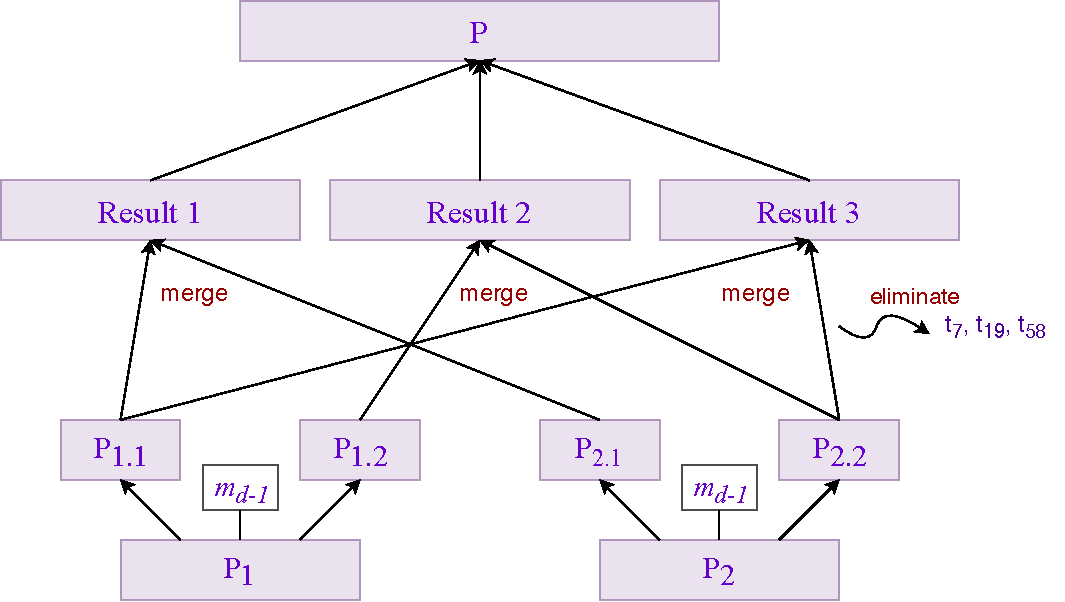
\includegraphics[width=0.9\linewidth]{figures/dnc-advanced-merge}
	\caption{DNC Advanced Merging}
	\label{fig:dnc-advanced-merge}
\end{figure}

% pseudo-code Divide-and-Conquer
\begin{algorithm}[h]
	\caption{Divide-and-Conquer Algorithm} \label{alg:dnc}
	\begin{algorithmic}[1] 
		\State \textbf{Input :} Tuple List $T$, Dimension $dim$
		\State \textbf{Output :} Skyline $skyline$
		\If {$T.size$ = 1} \textbf{return} $T$
		\EndIf
		\State $pivot \gets median$($T$, $dim$)
		\State ($P_{1},~P_{2}$) = $partition$($T$, $dim$, $pivot$)
		\State $S_{1} \gets$ Skyline($P_{1},~dim$)
		\State $S_{2} \gets$ Skyline($P_{2},~dim$)
		\State $merge\_result$ = $merge$($S_{1},~S_{2},~dim$)
		\State Add $S_{1}$ to $skyline$
		\State Add $merge\_result$ to $skyline$
		\State \textbf{return} $skyline$
	\end{algorithmic}
\end{algorithm}

% mway modification
For databases with limited main memory capacities the authors further suggest a modification to the basic DNC algorithm called \textit{M-way partitioning}. The main idea is to always partition the dataset in $M$ subsets instead of only two. $M$ should be chosen so that the size of the resulting partitions is small enough to fit into main memory. This approach has to be applied both during the partitioning phase as well as during the merging phase of the algorithm. This sort of modification, however, is not subject of this paper due to the context of in-memory databases. The M-way partitioning can be read up in more detail in \cite{kossmann}. 

%* DNC's worst-case complexity equals its best-case complexity\footnote{Which is $O(n~*~(log~n)^{d-2})~+~O(n~*~log~n)$.}~\cite{kossmann}. Therefore, the algorithm should only be taken in consideration when a high amount of ``worst-case scenarios'' is anticipated. 
Just like the BNL algorithm, Divide-and-Conquer cannot produce its results progressively, meaning that it can only output any of the skyline tuples, once the entire computation of the skyline is completed~\cite{survey}. 

\subsection{Other Algorithms}
With BNL and DNC being two of the more basic algorithms, several of the later proposed approaches reuse and extend their ideas, while optimizing the computation in specific areas. In the following, some of the newer skyline algorithms will be briefly introduced. 

% Bitmap, Index(index-based)
\subsubsection{Bitmap and Index Algorithms} \label{subsection:bitmap-index}
Bitmap \cite{bitmap-index} and Index \cite{bitmap-index} are two different algorithms aimed at producing the skyline tuples progressively while keeping response times generally low. 
The main idea of the Bitmap algorithm is to encode the underlying dataset as a bitmap structure in order to speed up computation \cite{survey}. In particular, the fact that bitwise operations are generally fast is exploited. At the beginning of the algorithm every single tuple from the underlying dataset has its attributes mapped into a bit-vector. Later, during computation, all comparison operations are executed on bit-slices derived from the bit-vectors. This enables the algorithm to quickly determine which tuples are dominated by others and which are not. 

The Index algorithm takes a different approach at progressive skyline computation and makes use of an index structure, namely a B$^{+}$-tree~\cite{bitmap-index}. In addition to that, while it does produce the skyline tuples progressively, it does not do so one-by-one, but does it in blocks instead~\cite{survey}. First, the algorithm implements a transformation mechanism which maps each tuple into one-dimensional space and stores it in the B$^{+}$-tree. During this process, tuples that are mapped to the same value are all stored in the same cluster. Due to the now existing sort order, the algorithm can decide which of the existing tuples are more likely to be part of the skyline, and therefore also behave more dominantly when eliminating other tuples. Also, tuples with common features that were previously mapped to land in the same cluster, can be checked for being part of the skyline in burst-like batches, which speeds up the performance and enables the algorithm to work progressively. 

% Nearest neighbor (NN), BBS (both with R* trees) both index-based
\subsubsection{NN and BBS Algorithms} \label{subsection:nn-bbs}
Another algorithm which is more focused on the ``big picture'' instead of the entire skyline, is the NN algorithm \cite{nn}. It is based on nearest-neighbor-search, hence the name. All the tuples of a dataset can be represented as $d$-dimensional points in a $d$-dimensional coordinate system. Assuming that the tuple attributes need to be minimized, the algorithm starts by applying nearest neighbor search to find the point that is closest to the origin. This point is inserted into the skyline right away. At this stage of the algorithm, it partitions the $d$-dimensional space of the coordinate system into four different partitions. The first one is the partition between the first point and the origin. It does not contain any further skyline points, as there are --- by definition of the nearest-neighbor-search --- no other points between the first one found and the origin. The second partition cannot contain any skyline points either, because they all have greater attribute values in every dimension than the first point, and are therefore dominated by it. The two remaining partitions can still contain points that are part of the skyline. The NN algorithm is recursively applied to these partitions for as long as there are any that are not empty. 

The nearest-neighbor-search component of the algorithm performs particularly well if the original dataset is indexed with a data structure such as the R*-tree. Just like the Bitmap and Index algorithms, the NN algorithm produces the skyline results progressively, i.e. without the need for the entire skyline to be computed before the first results are produced. While the first skyline tuples are output very fast, the rest of the skyline might need a much longer time to be computed \cite{nn}. 

A successor to the original NN algorithm, called BBS (Branch-and-Bound Skyline) \cite{bbs}, has been developed soon after. While it also makes use of the nearest-neighbor-search and the R*-tree, it has some significant improvements over the NN algorithm. One of these is that it only traverses the R*-tree once and thus reduces the number of redundant accesses. The algorithm organizes all of the skyline candidates in a heap and keeps them sorted according to their minimal distance from the origin \cite{survey}. There is more information on the BBS algorithm given in \cite{bbs}. 
%The first heap entry is the root of the R*-tree. In each iteration, the algorithm removes the entry at the top of the heap and does one of the following: 
%\begin{itemize}
%	\item If the removed heap entry is an inner node, then its not-dominated children are added to the heap and the next iteration of the algorithm starts. 
%	\item If the removed heap entry is a leaf node, then it is tested for being dominated, and if not inserted into the skyline.
%\end{itemize}

% Sort-filter-skyline (SFS) - sorting based BNL, Less is pretty similar, both sort-based
\subsubsection{Sorting-Based Algorithms} \label{subsection:sorting-based-algorithms}
There exists an entire range of sorting-based algorithms for skyline computation. The somewhat earlier developed SFS algorithm (Sort-Filter-Skyline) \cite{sfs} reuses the idea of the BNL algorithm and adjusts it so that the tuples are no longer considered in arbitrary order, but are instead presorted first. Then the tuples that are more likely to be part of the skyline are read in first. This way, the skyline can be computed faster, as the tuples inserted into the skyline at the beginning are very likely to be efficient ``tuple-killers'' and to eliminate most of the dominated tuples very fast. In addition to that, eligible tuples can be output progressively, which was not originally the case with the BNL algorithm. The drawback of presorting the underlying dataset is usually well compensated by the significantly reduced number of comparisons. 

% Less is too complex for such a minor improvement to list it here
%Another algorithm that shares its roots with BNL is LESS (Linear Elimination Sort for Skyline)(ref less). Just like the SFS algorithm, it presorts the original dataset, preferably with a special entropy scoring function. The authors suggest to hold an \textit{elimination filter} window with the most dominant tuples during the first pass of the external sorting function. This enables to discard dominated tuples fairly quickly. 

% SaLSa - based on SFS and LESS, direct predecessor of ST-S, sort-based
A further improvement over the SFS algorithm is its successor SaLSa (Sort and Limit Skyline Algorithm) \cite{salsa}. Just like SFS, it presorts the original dataset. However, this does not only happen for the reason of reducing the entire number of comparisons during computation. The key idea of SaLSa is to implement a threshold mechanism to stop the algorithm early as soon as all the tuples left are dominated by the tuples already in the skyline. In order to enable this technique, a slightly different sorting function is suggested, which works as following: First, all the tuples are presorted (ascending) according to their smallest attribute value among all dimensions. Then, if two or more tuples compete for the same position in the sorted set, the one with the smaller sum of attribute values across all dimensions wins the tie and gets the lesser position in the set. 

Later, during each iteration of the algorithm, the threshold value is updated with respect to the newest tuple that was read in. As soon as the stopping condition is reached, all tuples that are left, are dominated by the threshold, and the algorithm terminates. The stopping mechanism will be discussed in more detail in chapter \ref{subsection:sts}. 
Unfortunately, the threshold only reduces the number of tuples processed by the algorithm, but is not as efficient in scenarios with high dimensionality \cite{survey}. 

\subsection{ST-S Algorithm} \label{subsection:sts}
%introduction
One of the newest skyline algorithms to date is the ST-S (Skyline using Tree Sorting-based) algorithm \cite{rahman}. It is based on SaLSa, which, in its turn, is based on BNL and SFS. Thus, ST-S also belongs to the ``family'' of sorting-based algorithms. Its main addition to the concept of SaLSa is an algorithm-internal indexing structure, which is similar to a radix tree. This special tree structure is called \textit{N-Tree} within this work. The main purpose of the N-Tree is to execute dominance checks much faster by reducing the overall amount of comparisons between tuples. There are two drawbacks to the tree-based dominance checks. The first one is that ST-S is only suitable for categorical attributes, because continuous attributes (e.g. \textit{double} values) would imply an almost infinite amount of possible categories, and thus far too many children for each of the inner nodes of the tree. The second disadvantage is the somewhat higher memory usage during computation, as the tree structure takes up some of the available space. Using a tree structure to store skyline candidates however means that no separate \textit{window}, like in the original BNL algorithm, is needed. The authors in \cite{rahman} claim that ST-S significantly outperforms its predecessor SaLSa for categorical attributes in terms of computation time. In chapter \ref{chapter:Evaluation} of this work, ST-S will be further compared to the Naive-Nested-Loops and SARTS algorithms. 

%algorithm explanation
While the authors of the original paper \cite{rahman} work with binary attribute values (i.e. each attribute is either 0 or 1), they also propose using more categories if needed in a specific use case. This paper makes use of this proposition for generality purposes and implements the tree variant with multiple possible categories. 
The resulting tree structure used in ST-S is shown in Fig.~\ref{fig:ntree}. Every inner node, including the root, has an array which can hold as many children as there are possible attribute values. Hence, if all the values in the set $S := \{0,~1,~2,~3,~4\}$ can be taken, then each of the tree nodes has an array of size $|S| = 5$ with up to 5 different children. Each path taken from the root to a leaf represents the assignment of attribute values of some particular inserted tuple(s). The IDs of the tuples are always saved in form of arrays within the leaves. In addition to that, each of the inner nodes contains two different score values --- a \textit{minScore} and a \textit{maxScore}. MinScore represents the smallest possible score that can be achieved within leaves reachable from the current node. MaxScore stores the highest possible score, respectively. An illustration of the nodes is given in Fig.~\ref{fig:nnode}. 

\begin{figure}[h]
	\centering
	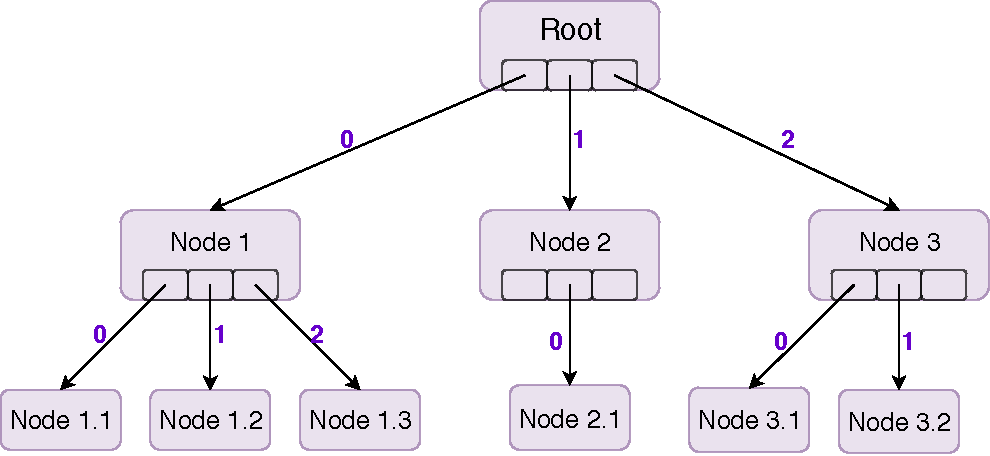
\includegraphics[width=0.8\linewidth]{figures/ntree}
	\caption{N-Tree for ST-S Algorithm}
	\label{fig:ntree}
\end{figure}

\begin{figure}[h]
	\centering
	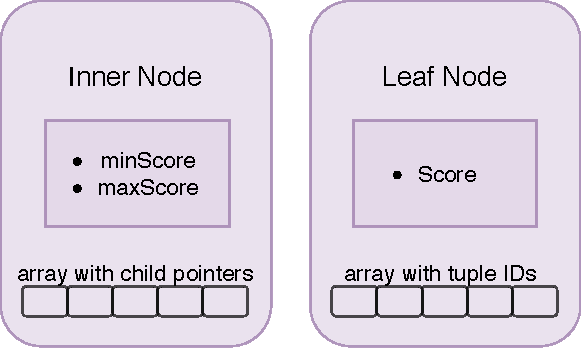
\includegraphics[height=0.3\linewidth]{figures/nnode}
	\caption{Nodes of the N-Tree}
	\label{fig:nnode}
\end{figure}

The score of a particular tuple is determined by a scoring function, let us call it $F$. The only condition that $F$ must fulfill is to not assign a higher score to a tuple that is dominated than to its dominator. The scoring function used in the following is 
\begin{equation}
F(t)~:=~\sum_{i~=~0}^{n-1}(2^{n~-~i}~*~t[A_{i}]), 
\end{equation}
with $t$ being the tuple to receive a score, $n$ the length of the tuple, and $t[A_{i}]$ the $i$-th attribute of the tuple. 

At the beginning, the tuples are sorted with the monotonic function \textit{minC()} (resp. \textit{maxC()} if the attributes have to be maximized). \textit{minC()} is defined as 
\begin{equation}
minC(t) := (min_{A_{i}}\{t[A_{i}]\},~\sum_{A_{i}}(t[A_{i}])).
\end{equation}
It consists of two components as mentioned in chapter \ref{subsection:sorting-based-algorithms}: a main comparison attribute, which is the smallest of all attribute values of a tuple, and a tie-breaker being the sum over all attribute values of the same tuple. Suppose the dataset shown in Fig.~\ref{fig:minc}~(a). By applying the sorting function \textit{minC} to the dataset, the sorted list of tuples shown in Fig.~\ref{fig:minc}~(b) emerges. 

\begin{figure}[h]
	\centering
	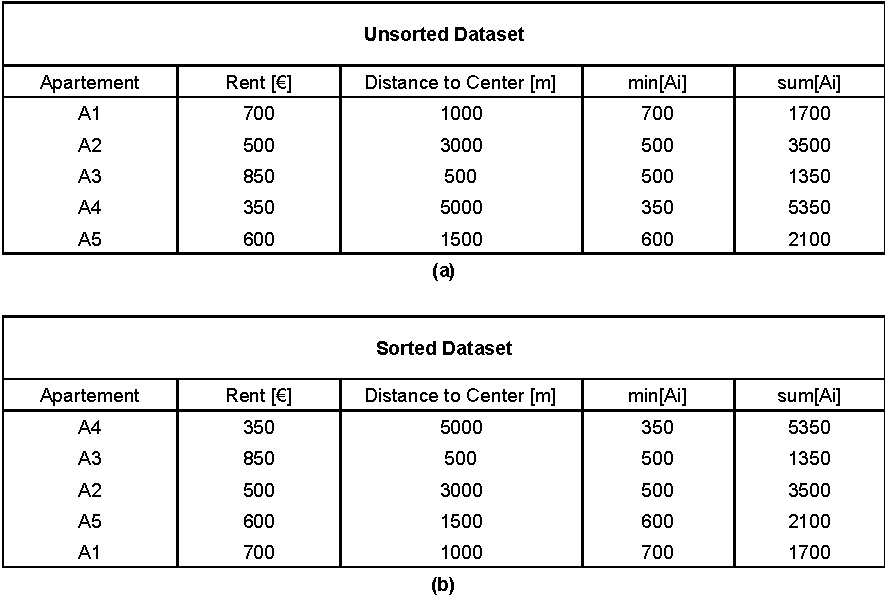
\includegraphics[width=0.95\linewidth]{figures/minc}
	\caption{Example: Sorting with \textit{minC()}}
	\label{fig:minc}
\end{figure}

The pseudo-code to the ST-S algorithm is given in Algorithm \ref{alg:sts}. It works as following: 
\begin{enumerate}
	\item The tuples are presorted with \textit{minC()} (line 3).
	\item $t_{stop}$ is the threshold, and is undefined at the beginning. It is later updated (lines 13-14) with knowledge of some tuples that have been proved to be part of the skyline. 
	\item The first tuple $t_{0}$ from the presorted dataset is always part of the skyline due to the choice of \textit{minC()}. It gets inserted into the tree and is put out as part of the skyline (lines 5-7). 
	\item In the following loop every tuple $t$ of the sorted dataset, except for the first one $t_{0}$, is checked for being dominated by any tuple already in the skyline (line 10). The checks are carried out with the help of the tree, which holds all the skyline tuples to date. The responsible operation \textit{is\_dominated} will be introduced in more detail later. 
	\item If a tuple $t$ is dominated by some other tuple in the skyline, it is no longer considered for the skyline. If it is not dominated, it gets inserted into the tree (line 11), so that it is able to eliminate future tuples that are not part of the skyline. 
	\item If the maximum attribute value of the new skyline tuple $t$ is smaller than the maximum attribute value of the threshold $t_{stop}$, then the threshold is updated (line 14), and now holds the value of $t$, until the next update occurs. 
	\item At the beginning of each iteration of the loop, the stopping condition is checked (line 9), so that the algorithm can stop early if all the tuples left in the dataset are \`{a}-priori dominated by the threshold. This functionality has been inherited from the SaLSa algorithm (chapter \ref{subsection:sorting-based-algorithms}). If the maximum attribute value of the threshold tuple $t_{stop}$ is less or equal to the minimum attribute value of the current tuple $t$, and the two tuples are not the same, then thanks to presorting with \textit{minC()} none of the remaining tuples can be part of the skyline. At this point, the algorithm can terminate and the tree with the tuples is no longer needed. If the tuples are the same, however, then the current tuple also has to be checked to be part of the skyline. 
\end{enumerate}

% pseudo-code ST-S
\begin{algorithm}[h]
	\caption{ST-S Algorithm} \label{alg:sts}
	\begin{algorithmic}[1] 
		\State \textbf{Input :} Tuple List $T$, Tree $tree$
		\State \textbf{Output :} Skyline $skyline$
		\State Sort $ T $ in-place using a monotonic function \textit{minC()}
		\State $t_{0} \gets $ first element of $T$
		\State $t_{stop} \gets t_{0}$
		\State insert($t_{0}$, $tree.root$, 0)
		\State Add $t_{0}$ to $skyline$ $~~~~~$ {\footnotesize // $t_{0}$ always part of skyline due to presorting}
		\For {each tuple $t~\in~T\backslash\{t_{0}\}$}
			\If {$max$($t_{stop}$)$~\leq~min$($t$) and $t_{stop}~\neq~t$}
				\textbf{return}
			\EndIf
			\If {\textbf{not} is\_dominated($t$, $tree.root$, 0, $score(t)$)}
				\State insert($t$, $tree.root$, 0)
				\State Add $t$ to $skyline$
				\If {$max(t)~<~max(t_{stop})$}
					\State $t_{stop} \gets t$ 
				\EndIf
			\EndIf
		\EndFor	
	\end{algorithmic}
\end{algorithm}

\noindent Both the \textit{insert} and \textit{is\_dominated} operations have been slightly modified from the original variant, in order to incorporate multiple attribute categories instead of just two. They also make use of the \textit{minScore} and \textit{maxScore} functionality to speed up dominance checks within the tree. 

The pseudo-code to the \textit{insert} operation is shown in Algorithm \ref{alg:sts-insert}. The proceedings are the following: 
\begin{enumerate}
	\item Depending on the current depth level within the tree, the \textit{minScore} and \textit{maxScore} attributes of the current node are updated (lines 2-7). On level 0 (root level) the smallest possible score is 0, and the highest possible score is calculated using the greatest-possible attribute value for each of the remaining levels. If the current node is not the root, the scores are updated by applying the scoring function in accordance with the current tree level and the attribute values which already occured. 
	\item If the current level is the deepest level possible, then it means that the algorithm reached a leaf node (line 8). At this point, if some other tuple has already been inserted in this leaf node, the score of the leaf no longer needs to be calculated. If the current tuple is the first one to get stored in the leaf, then the node's score is updated. In any case, the \textit{tupleID} of the tuple is attached to the \textit{tupleIDs} list of the leaf node (lines 9-10). 
	\item If the last level has not yet been reached, then the tree has to be further traversed. For this purpose, the \textit{insert} operation is called recursively on the child node at position $t[level]$ with the same tuple $t$ and the \textit{level} increased by one (line 15). 
	\item If the child at the position $t[level]$ does not yet exist, it is simply created as a new node (lines 13-14) before further traversing the tree. 
\end{enumerate}

% pseudo-code INSERT
\begin{algorithm}[h]
	\caption{INSERT Operation for ST-S} \label{alg:sts-insert}
	\begin{algorithmic}[1]		
		\State \textbf{Input :} Tuple $t$, Node $node$, Level $level$, Attributes $atts$
		\If {$level$ = 0}
			\State $node.minScore \gets 0$
			\State $node.maxScore \gets \sum_{i~=~0}^{t.size~-~1}(2^{t.size~-~i}~*~max(atts))$
		\Else 
			\State $node.minScore \gets \sum_{i~=~0}^{level~-~1}(2^{t.size~-~i}~*~t[i])$
			\State $node.maxScore \gets node.minScore~+~\sum_{i~=~level}^{t.size~-~1}(2^{t.size~-~i}~*~max(atts))$
		\EndIf
		\If {$level$ = $t.size$} 
			\If {$node.score$ is $None$}
				\State $node.score \gets score(t)$
			\EndIf
			\State Append $t.tupleID$ to $node.tupleIDs$
		\Else
			\If {$node.child[t[level]]$ \textbf{not} exists}
				\State $node.child[t[level]] \gets New$ Node()
			\EndIf
			\State insert($t$, $node.child[t[level]]$, $level~+~1$)
		\EndIf
	\end{algorithmic}
\end{algorithm}

\noindent The pseudo-code to the \textit{is\_dominated} operation can be seen in Algorithm \ref{alg:sts-is-dominated}. Starting from the root, the tree is traversed from top to bottom. The usage of the sorting and scoring functions enables the algorithm to only search in those branches of the tree that are not \`{a}-priori dominated. 
\begin{enumerate}
	\item In this work the wish to minimize the attribute values is assumed. Therefore, only those children of the current node that have a smaller position than $t[level]$ are further considered in the dominance test. These children are recursively traversed by the \textit{is\_dominated} function (lines 7-11). 
	\item If the current node is \textit{None}, then it has not yet been initialized, and thus also does not have any children that the algorithm could traverse. Hence, there are no paths from the current node that would dominate the given tuple. \textit{False} is returned (line 3). 
	\item Also, if the score of the given tuple is smaller than the smallest-possible score of the current node, then, due to our choice of the scoring function, the tuple cannot be dominated by any path through this node. \textit{False} is returned (line 3). 
	\item If by traversing the tree the deepest possible \textit{level} has been reached, the algorithm checks whether the score of the given tuple equals the score of the leaf node. If the scores are equal, then the tuple is obviously not dominated by the other tuples in this leaf node, and \textit{False} is returned (line 5). Otherwise, \textit{True} is returned and the tuple is no longer considered a skyline candidate (line 6). 
\end{enumerate}

% pseudo-code IS_DOMINATED
\begin{algorithm}[]
	\caption{IS\_DOMINATED Operation for ST-S} \label{alg:sts-is-dominated}
	\begin{algorithmic}[1]		
		\State \textbf{Input :} Tuple $t$, Node $node$, Level $level$, Score $s$
		\State \textbf{Output :} True if $t$ is dominated, otherwise False
		\If {$node$ is $None$ or $s < node.minScore$} \textbf{return} False
		\EndIf
		\If {$level = t.size$ and $score(t)~\neq~node.score$} \textbf{return} True
		\EndIf
		\If {$level = t.size$ and $score(t)~=~node.score$} \textbf{return} False
		\EndIf
		\State $weight \gets 2^{t.size~-~level}~*~t[level]$
		\For {each $i~\in~N_{0},~i~<~t[level]$}
			\If {is\_dominated($t$, $node.child[i]$, $level~+~1$, $s~+~weight$)}
			\State \textbf{return} True
			\EndIf
		\EndFor
		\If {is\_dominated($t$, $node.child[t[level]]$, $level~+~1$, $s$)}
		\State \textbf{return} True
		\EndIf
		\State \textbf{return} False
	\end{algorithmic}
\end{algorithm}

% If not enough content, also cover ST-P and TA-SKY

\subsection{Classification} \label{classification}
The previously introduced skyline algorithms can be organized according to different criteria. %, such as their basic idea, the algorithms they are related to, as well as whether they can produce results progressively or not \cite{survey}. 
A classification with criteria related to the topic of this work is given in Table~\ref{fig:classification}. 

\begin{figure}[h]
	\centering
	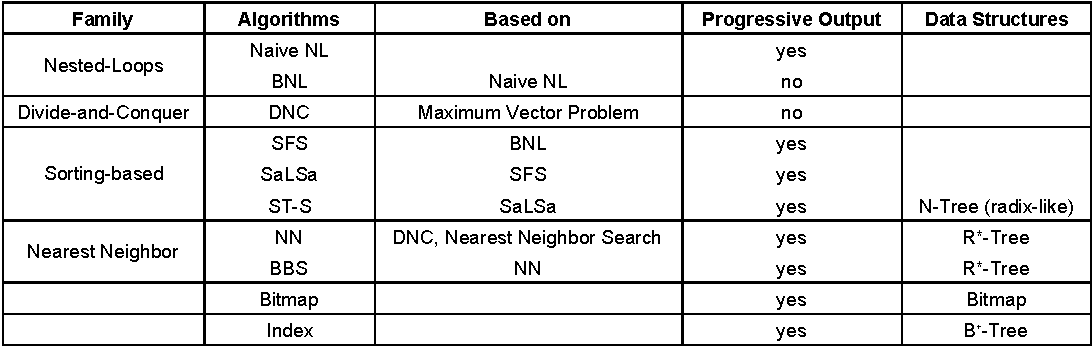
\includegraphics[width=1\linewidth]{figures/classification}
	\captionof{table}{Classification of Introduced Algorithms}
	\label{fig:classification}
\end{figure}

\subsection{Parallelization Approaches} \label{subsection:parallelization-approaches}
%While applications can generally be parallelized with the help of GPUs, multicore CPUs, as well as in distributed environments, such as MapReduce \cite{book-kemper}, 
The focus of this work lies within multicore parallelization with CPUs. In the following, some of the modern approaches to parallelization of skyline algorithms are briefly covered. 

\subsubsection{Parallelization Criteria} \label{subsection:parallelization-criteria}
Chester et al. \cite{chester} (2015) propose in their work on skyline parallelism the main criteria for developing efficient multicore parallelization approaches. The key suggestions are: 
\begin{enumerate}
	\item When dividing the input data into subsets, the resulting data blocks should be independent, unordered, and about equal-sized. This way, the results of each working unit will not depend on the results of other units and the workload will be close to equally distributed. 
	\item Data structures that are shared between threads should be either in read-only mode, or only have a few write changes during parallelization. While the coordination on write accesses could be achieved by locking, this often results in a major bottleneck of the otherwise parallel execution. If the number of writes is high and no locks are used, race conditions between threads are almost certain to occur. 
	\item If synchronization points are used, their location in the code should be chosen very carefully. At these points, there is no parallel processing both during the time of waiting for the single threads to finish their current work, and during the time of sequential synchronization. If the synchronization points were chosen wrongly, the performance of the algorithm will most certainly take a significant hit. 
\end{enumerate}

%\subsubsection{Parallelizing BBS} \label{subsection:parallelizing-bbs}
%Park et al. \cite{parallel-bbs} (2011) made successful use of \textit{skeletal parallel programming} \cite{skeletal} when parallelizing the previously mentioned BBS algorithm (chapter \ref{subsection:nn-bbs}). 
%For this purpose the authors used the OpenMP~\cite{openmp} parallelization framework, which parallelizes given regions of the program by issuing compiler directives. Parallelization with OpenMP is usually relatively well applicable to already existing sequential programs, as adding compiler directives to parallelizable regions of the code usually does not imply any significant code changes. For a naive parallelization approach, Park et al. identified the two most computation-intensive parts of the program and simply annotated them with OpenMP parallelization directives. However, this did not produce the desired speedup of the algorithm. The reason for this was that the parallel-running threads are not per-se able to exchange information on already eliminated tuples and thus the entire number of comparisons per skyline significantly rises. OpenMP does not allow the programmer to stop threads by \textit{break} command or equals during runtime\footnote{I.e. it issues compilation errors. This was checked in the scope of this work.}. Enabling explicit communication patterns between threads would slow the program down significantly as explained earlier in this chapter. 
%
%% TODO right now the solution doesnt make too much sense
%The solution was to first gather the incomparable candidate tuples, and afterwards to inspect these in parallel using \textit{tbb's parallel\_for}~\cite{parallel-for} construct. 
%This paper will further consider OpenMP and tbb's parallel\_for as parallelization frameworks for the relevant skyline algorithms (chapter \ref{chapter:Parallelization}). 

% specially developed parallel skyline algorithms
\subsubsection{Existing Parallel Algorithms} \label{subsection:other-parallel-algorithms}
%Only a few of the existing sequential algorithms have been parallelized so far. One of these is the previously mentioned BBS algorithm for instance. In their work, Park et al. made successful use of \textit{tbb's parallel\_for}~\cite{parallel-for} construct after identifying the regions in their code suitable for parallelization \cite{parallel-bbs}. Their first attempt to parallelize the critical regions with OpenMP~\cite{openmp}, however, failed as the parallelization was not able to improve the computation time of the initial algorithm. In this work, OpenMP and tbb's parallel\_for will be further considered as parallelization frameworks for the relevant skyline algorithms. 

A range of new algorithms, specifically developed for parallel execution, has recently appeared. Some of the interesting ones to read up on include \textit{pskyline}~\cite{parallel-bbs} and \textit{APSkyline}~\cite{apskyline} based on the divide-and-conquer principle, \textit{Hybrid}~\cite{chester} making use of prefiltering, partitioning, and sorting, \textit{SkyAlign}~\cite{skyalign}, which is one of the few skyline algorithms specifically designed for GPU computation, as well as \textit{MR-GPMRS} \cite{map-reduce} designed for computation with the MapReduce paradigm. This paper will not discuss these algorithms in greater detail, as it is more aimed at parallelizing existing sequential algorithms, as well as the novel SARTS algorithm (chapter \ref{chapter:ARTforSkyline}). 




%One of the main achievements of Kung et al. was probably to determine the theoretically applicable upper bounds for the number of comparisons a skyline algorithm might have to perform. These boundaries apply to the worst-case scenario. With $C_{max}$ being the maximum number of comparisons, $n$ the number of vectors, and $dim$ the number of dimensions of each vector, according to Kung et al. we receive: 
%\begin{equation}
%C_{max}(n) = n - 1 for dim = 1, 
%\end{equation}
%\begin{equation}
%C_{max}(n) \leq O(n log n) for dim = 2,3,  
%\end{equation}
%\begin{equation}
%C_{max}(n) \leq O(n (log n)^{d-2}) for dim \geq 4, 
%\end{equation}


		\chapter{ART for Skyline} \label{chapter:ARTforSkyline}
%With ST-S being one of the most efficient state-of-the-art skyline algorithms for categorical attributes and in the absence of indexes, the question arises if the algorithm can be further improved. 
In the following, this work presents a novel skyline algorithm called SARTS, which beholds all of the major advantages of the ST-S algorithm, and further improves it by utilizing the more memory-efficient tree structure ART. 

\section{Adaptive Radix Tree} \label{section:art}
The Adaptive Radix Tree (ART) \cite{art} is an efficient indexing structure, specifically designed for main-memory databases. In contrast to most traditional in-memory indexing structures, like binary search trees, ART is able to make optimal usage of modern CPU caches, thus enabling both quicker response times and lower space consumption. The main difference to traditional radix trees is the adaptive resizability of the tree's inner nodes, which results in much more compact tree design. 

\subsection{Characteristics} \label{section:art-characteristics}
%Radix trees have several advantages over comparison based trees, like e.g. binary search trees. The most important ones are: 
%\begin{itemize}
%	\item Better scaling with the number of elements inserted, as the height of the tree depends on key length and not on the number of elements. 
%	\item No extra CPU usage for rebalancing operations is required. 
%	\item Implicit storage of the keys in form of the path taken to the particular element, and thus lower memory consumption. 
%\end{itemize}
The main drawback of radix trees is wasteful space behavior. The reason for this is that all inner nodes in the radix tree have child arrays of exactly the same size, independently of how many of the child pointers are not null. Therefore, if some of the children do not exist, the excessive memory needed to fully allocate the array of pointers is simply wasted. 

The ART tree solves this problem by introducing resizable nodes of four different types: \textit{Node4}, \textit{Node16}, \textit{Node48} and \textit{Node256}. The nodes can have up to 4, 16, 48 and 256 child pointers, respectively. Whenever an inner node has not enough space to insert a new child pointer, it grows to the next bigger type. Similarly, if one of the existing child nodes has been deleted from the tree, then its parent checks if the number of its children is small enough to shrink to the next smaller size. 

\begin{figure}[h]
\centering
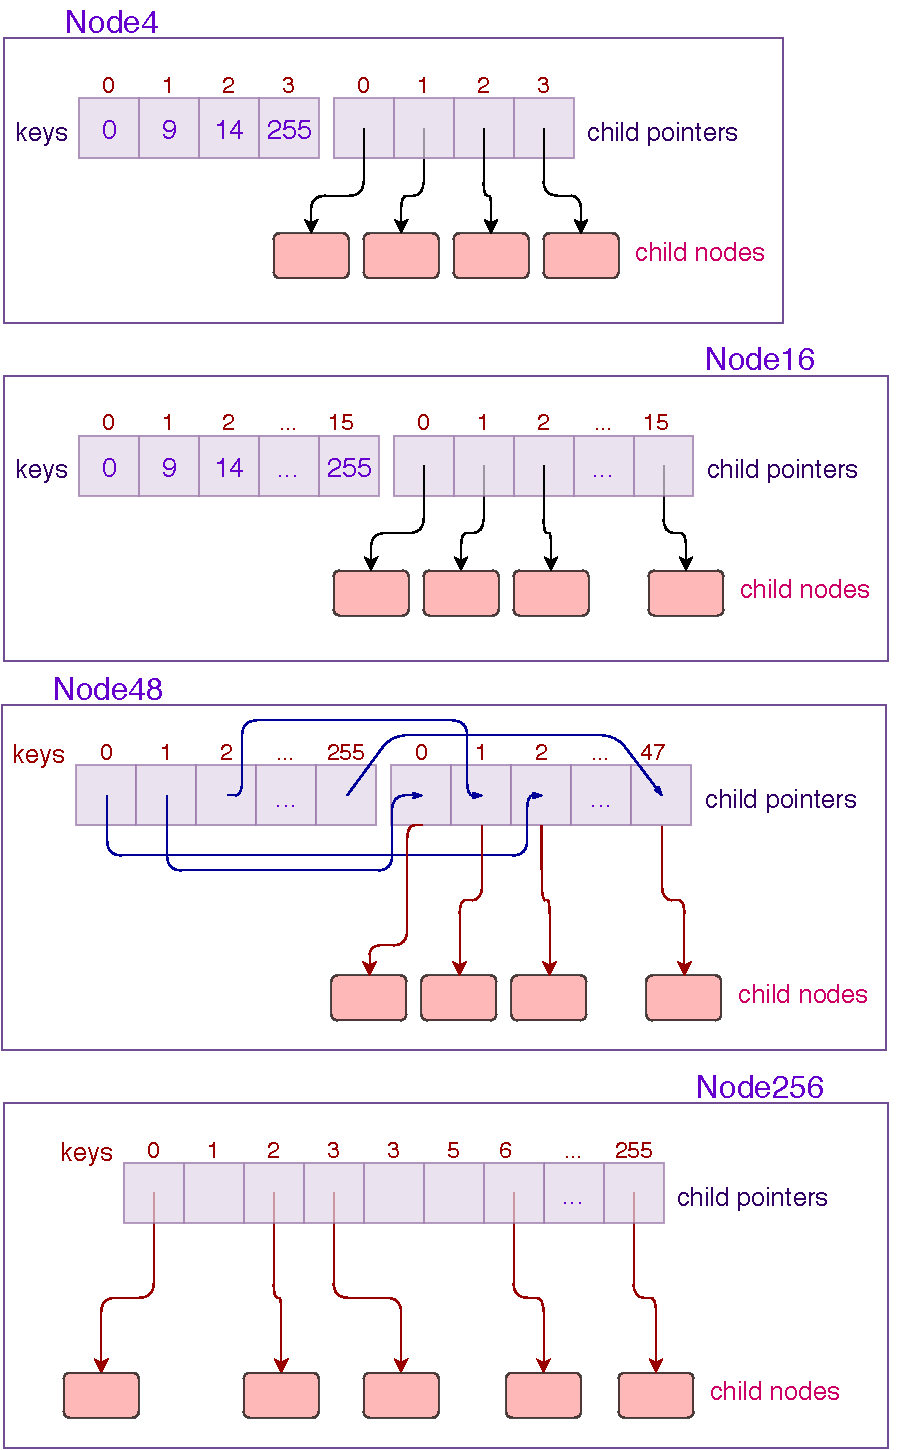
\includegraphics[width=0.8\linewidth]{figures/art-nodes}
\caption{Node Types of the ART Tree}
\label{fig:art-nodes}
\end{figure}

Each of the nodes consists of two different arrays, which function similarly to a key-value store. The entries in the keys array point to the corresponding entries in the array with child pointers. The structure of the four node types is illustrated in Fig.~\ref{fig:art-nodes} and described in the following: 
\begin{itemize}
	\item \textbf{Node4:} The first array is responsible for storing the key bytes in ascending order. The second array holds the pointers to the child nodes. Both arrays are of size 4. 
	\item \textbf{Node16:} This node type is the same as Node4, except for that its arrays are of size 16. 
	\item \textbf{Node48:} With 48 different entries, sequential search for the right entry in the keys array would take too much time. Therefore, Node48 implements a 256-element array for the key entries. Unlike Node4 and Node16, the key bytes now can be found directly in the index of the array, and the elements of the array are pointers to the entries in the children array. 
	\item \textbf{Node256:} This is the largest possible and also the simplest node type in the tree, and can hold up to 256 different entries. It only consists of one array. The key bytes can be found in the index of the array and the entries are child pointers. This way, no indirection is needed in this node type. 
\end{itemize}
In addition to that, each of the nodes possesses a header which holds attributes such as the node type and the number of its chidren. This list of attributes can be adjusted depending on the particular use case of the ART tree. Chapter \ref{section:sarts} makes use of such adjustments. 

Due to the complex structure of the ART nodes, special operations are needed to make use of them. These include \textit{findChild}, \textit{newNode} and \textit{grow}. The operations are explained in greater detail in \cite{art}; the C++ code to each of them can be found in Appendix \ref{appendix-code} to this work. 

%\subsection{Core Algorithms} \label{section:art-algorithms}
%In this section, some of the most important operations that are part of the ART tree are explained. The full C++ code to each of them can be found in the appendix to this work (section \ref{appendix-code}). 
%% Insert
%To begin with \textit{insert}, its main functionality is the following: 
%\begin{enumerate}
%	\item Starting from the root (which is the size of Node4 initially), the first key byte of the new tuple is taken. 
%	\item Depending on the current node type, the corresponding child pointer is found. If the child does not yet exist, then the pointer is null. 
%	\item If the child pointer is null, the node checks if it needs to grow in order to insert a new child. If it has to --- it does, if not --- it does not. The new child is created and a pointer to it is stored in the children array. 
%	\item The edge to the next node is followed. 
%	\item The procedure repeats recursively, until the last byte of the key has been used. At this point, the tuple (and the information within it) is inserted into a leaf node. The key bytes of the tuple do not need to be stored explicitly. 
%\end{enumerate}
%
%% findChild
%\noindent Finding the right child within a node depends on the type of the current node. This is how the \textit{find\_child} function works:
%\begin{itemize}
%	\item \textbf{Node4:} The keys array is traversed until the element is found that corresponds the key byte entry of the given tuple. The index of this element is now the index of the child pointer in the children array. If the pointer is null, then no such child exists yet. In any case, the child pointer is returned. Both arrays are traversed sequentially as the array size is too small to require more efficient searching techniques. 
%	\item \textbf{Node16:} The keys array of Node16 is bigger than that of Node4. Therefore, it is sensible to utilize some faster searching technique than simply traversing the array from left to right. The authors in \cite{art} propose to either use binary search or SIMD\footnote{Single Instruction, Multiple Data} instructions to speed up the search. As soon as the index of the given key byte is found, the child pointer under this index can be returned, just like in Node4. 
%	\item \textbf{Node48:} The given key byte is taken as the index of the keys array. The element stored under this index is the needed index of the children array. If the element is marked as empty (e.g. with the value 48 in the entry\footnote{The value 48 is vacant, because the keys array of Node48 only holds values between 0 and 47 due to the size of its children array.}), then the function returns a null pointer. Otherwise, the child pointer under this index is returned as the next node. 
%	\item \textbf{Node256:} The given key byte is the index of the needed child entry. The child entry is returned either as a node pointer or a null pointer.  
%\end{itemize}
%
%% newChild
%\noindent Every new child node that is created is always of the smallest-possible Node4 type, because it is empty at the beginning. Creating a new child, however, is still node-type-dependent. The functionality is introduced in the following: 
%\begin{itemize}
%	\item \textbf{Node4 \& Node16:} To find the correct position for the new key entry, the keys array, which is sorted in ascending order, is traversed, until the correct position for the new key byte is found. If this position is already taken, then it is freed by moving all the hindering entries one slot to the right. The same happens with the children array to keep the correct indexing order. Now the new key byte and the new child pointer are added under the same index to the respective arrays. 
%	\item \textbf{Node48:} The new child is added in the first free slot of the children array. Then, a pointer to this slot is saved in the keys array at the index that equals the new key byte. 
%	\item \textbf{Node256:} The new child is simply added at the position with the index that equals the new key byte. 
%\end{itemize}
%
%% grow
%\noindent Growing a node with the \textit{grow} operation is relatively straightforward: 
%\begin{enumerate}
%	\item A new node of the next-bigger type is created. 
%	\item The key bytes, the child pointers as well as any other information stored in the current node are copied into the new node. 
%	\item The parent of the current node gets updated about the new child. Its pointer now points to the new child. 
%	\item The current node is deleted to avoid potential misunderstandings and to free now unused memory. 
%\end{enumerate}

% path compression and lazy expansion
\subsection{Further Optimizations} \label{section:art-further-optimizations}
In addition to the core functionality of ART, the authors propose two further optimizations. The first one is called \textit{lazy expansion}. With this technique, inner nodes are only created if there is more than one path to the leaves passing through them. Otherwise, they are simply left out to save space and to reduce access time to the leaves. The second technique is called \textit{path compression}. It results in removing all inner nodes that only have one child node. %Since the part of the key which was previously stored in preceding inner nodes now misses, some workarounds, such as storing partial key vectors at inner nodes, are necessary to make this technique work. 
Both lazy expansion and path compression could be useful when trying to save even more space and to improve lookup times. More details on both techniques are provided in \cite{art}. 

\section{SARTS - A Novel Skyline Algorithm} \label{section:sarts}
%idea
In the following, SARTS (Skyline using ART Sorting-based), a novel skyline algorithm for categorical attributes is presented. It makes use of the core concepts of ST-S (chapter \ref{subsection:sts}), and further improves it by implementing a more efficient indexing structure for dominance checks --- the ART tree. 

% approach
The interface of the ART tree has been kept similar to that of the N-Tree in ST-S. This enables for a very straightforward integration of the ART tree into the algorithm, because the \textit{insert} and \textit{is\_dominated} operations still have the same signature as in ST-S. While \textit{insert} is slightly different from the original variant on the inside, the \textit{is\_dominated} operation is almost identical to the one in ST-S. Therefore, for the pseudo-code of SARTS and \textit{is\_dominated} it can be referred to Algorithms \ref{alg:sts} and \ref{alg:sts-is-dominated}. 

% pseudocode insert
The \textit{insert} operation for SARTS differs from the ST-S variant in that both finding the correct child to the current node and creating a new child are outsourced into two separate functions: \textit{findChild()} and \textit{newChild()}. In addition to that, before a new child can be created, the current node might first need to \textit{grow()} to the next-bigger type, in order to create space for the new child. The pseudo-code to the \textit{insert} operation is given in Algorithm \ref{alg:sarts-insert}.
\begin{algorithm}[h]
	\caption{INSERT Operation for SARTS} \label{alg:sarts-insert}
	\begin{algorithmic}[1]		
		\State \textbf{Input :} Tuple $t$, Node $parent$ Node $current$, Level $level$, Attributes $atts$
		\If {$level$ = 0}
			\State $node.minScore \gets 0$
			\State $node.maxScore \gets \sum_{i~=~0}^{t.size~-~1}(2^{t.size~-~i}~*~max(atts))$
		\Else 
			\State $node.minScore \gets \sum_{i~=~0}^{level~-~1}(2^{t.size~-~i}~*~t[i])$
			\State $node.maxScore \gets node.minScore~+~\sum_{i~=~level}^{t.size~-~1}(2^{t.size~-~i}~*~max(atts))$
		\EndIf
		\If {$level$ = $t.size$} 
			\If {$node.score$ is $None$}
				\State $node.score \gets score(t)$
			\EndIf
			\State Append $t.tupleID$ to $node.tupleIDs$
		\Else
			\State $child \gets findChild$($current$, $t[level]$)
			\If {$child$ is $None$}
				\If {$current.size$ = 4 \textbf{or} $current.size$ = 16 \textbf{or} $current.size$ = 48}
					\State $grow$($parent$, $current$, $t[level~-~1]$)
				\EndIf
%				\Switch {$current.type$}
%					\Case {Node4}
%						\If {$current.size$ = 4}
%							\State $grow$($parent$, $current$, $t[level~-~1]$)
%						\EndIf
%					\EndCase
%					\Case {Node16}
%						\If {$current.size$ = 16}
%							\State $grow$($parent$, $current$, $t[level~-~1]$)
%						\EndIf
%					\EndCase
%					\Case {Node48}
%						\If {$current.size$ = 48}
%							\State $grow$($parent$, $current$, $t[level~-~1]$)
%						\EndIf
%					\EndCase
%				\EndSwitch
				\State $child \gets newChild$($current$, $t[level]$)
			\EndIf
			\State insert($t$, $current$, $child$, $level~+~1$)
		\EndIf
	\end{algorithmic}
\end{algorithm}

% pseudocode is dominated
The main difference within the \textit{is\_dominated} operation is, similarly to \textit{insert}, the usage of the \textit{findChild()} function any time the correct child for further traversing of the tree needs to be found. 

In addition to that, just like the nodes of the N-Tree, the inner nodes of the ART tree have to be extended by a \textit{minScore} and a \textit{maxScore}, and the leaf nodes by the \textit{score} attribute and an array of \textit{tupleIDs}. This enables faster traversing of the tree during dominance checks by skipping tree regions that cannot dominate the current tuple. 

% The ART version taken
The ART version used in this paper is the basic one for simplicity purposes. It does not incorporate the two optimization approaches \textit{path compression} and \textit{lazy expansion}. 


		\chapter{Parallelization} \label{chapter:Parallelization}
The following chapter presents the parallelization approaches suggested in this work. %These include some of the more ``traditional'' skyline algorithms, such as Naive-Nested-Loops and DNC, as well as two of the newer algorithms ST-S and SARTS. 
All the algorithms were implemented and parallelized in C++, mainly due to its efficiency in terms of speed and memory management. 

\section{Methods and Frameworks} \label{section:methods-frameworks}
There are two different implementation models used for the algorithms. The Block-Nested-Loops algorithm is implemented in two versions: one of them makes use of the Volcano model, the other of the produce/consume concept. This was done in order to be able to compare the two models in terms of their performance. The rest of the algorithms were implemented with the produce/consume concept only. Both models are briefly covered in the following. 

% volcano style
\subsection{Volcano Model}
The Volcano Model, sometimes also called Iterator Model, is an evaluation strategy of database queries \cite{volcano-wiki}. A standard database query is evaluated by passing a stream of tuples through several database operators, with each of these operators doing their task (e.g. join, filter, skyline, etc.). Whenever an operator calls \textit{next()} on its predecessor in the evaluation pipeline, the preceding operator has two options: 
\begin{itemize}
	\item If the next tuple is ready to be delivered, it is simply returned. 
	\item If the next tuple has not yet been produced, then the predecessor either produces it itself, or, if necessary, first calls \textit{next()} on its own preceding operator. 
\end{itemize}
The query pipelining process for the Volcano Model is visualized in Fig.~\ref{fig:volcano-model}. In some cases, the response time to a \textit{next()} call can be fairly long due to the requested tuple(s) not being ready for delivery yet. %Suppose a database query which consists of two tasks. First, the tuples from the underlying set of apartments have to be filtered, so that only apartments under 1000 euros rent are considered. Second, the skyline of the resulting set of apartments has to be computed. In this case, as soon as the skyline operator calls \textit{next()} on the selection operator, the latter starts filtering the underlying dataset. It is only after the filtering that it returns the requested tuples to the call issued by the skyline operator. After that, the skyline of the apartments is computed, and the result of the query is issued. 

%The main advantages of the Volcano evaluation strategy are that Volcano is easily ``extensible with new operators, algorithms, data types, and type-specific methods'' \cite{volcano}. 

\begin{figure}[h]
	\centering
	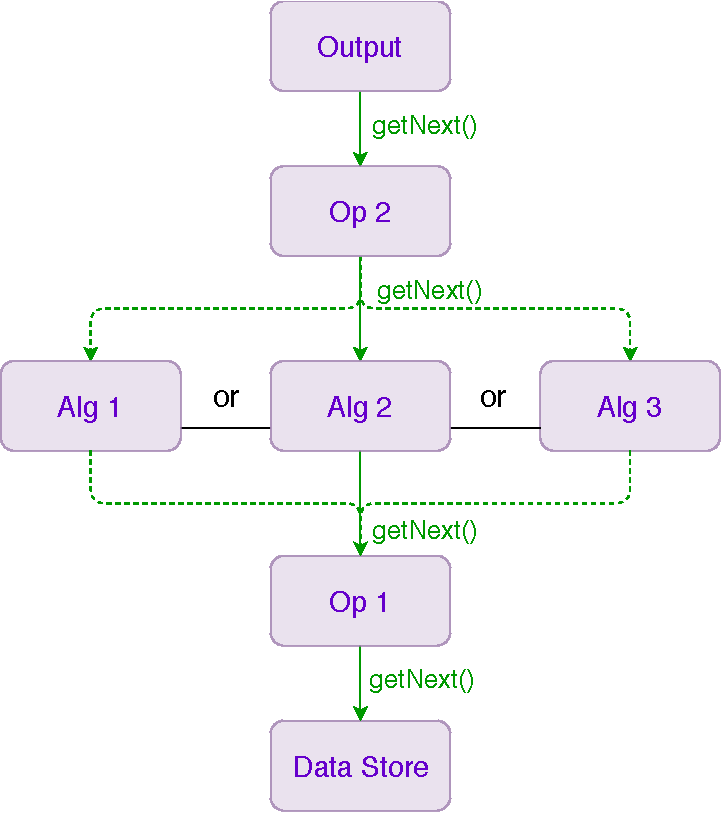
\includegraphics[height=0.6\linewidth]{figures/volcano-model}
	\caption{Query Pipelining with Volcano Model}
	\label{fig:volcano-model}
\end{figure}

% produce/consume
\subsection{Produce/Consume}
The produce/consume concept is slightly different. Each of the database operators has one child operator and one parent operator. All operators implement the common \textit{operator} interface, and thus all possess a child, a parent, as well as the two functions \textit{produce} and \textit{consume}. Whenever an operator needs its child to produce tuples, it calls \textit{produce} on the child. This only happens once, and therefore prevents the operator from continuously calling \textit{next} as it is the case in the Volcano model. After the child received the produce instruction, it first calls \textit{produce} on its own child. As soon as all the tuples have been received and processed, the child repeatedly calls \textit{consume} on its parent and ``feeds'' the tuples to it one by one. The entire process is shown in Fig.~\ref{fig:produce-consume-model}. %There are only as many \textit{consume()} calls as there are tuples to transfer between every two operators. The produce/consume concept, however, is only used during code generation and does not exist at runtime. Just like the volcano model, produce/consume also allows for an easy exchangeability of operators and algorithms, as these can be easily integrated into the query evaluation pipeline \cite{produce-consume}. %TODO: Leave this out?

\begin{figure}[h]
	\centering
	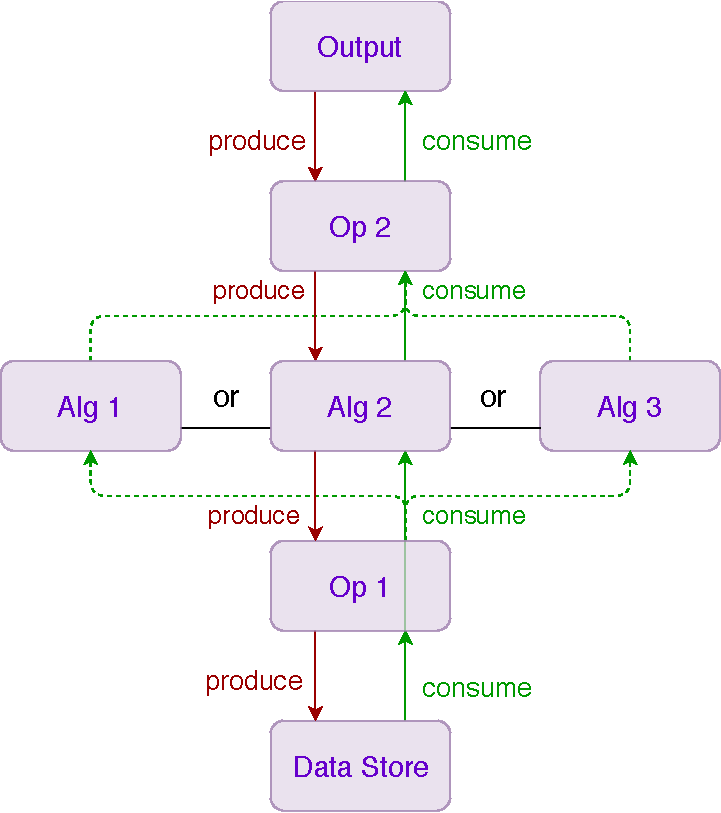
\includegraphics[height=0.6\linewidth]{figures/produce-consume-model}
	\caption{Query Pipelining with Produce/Consume Model}
	\label{fig:produce-consume-model}
\end{figure}

It is important to notice that the produce/consume concept used in this work does \textbf{not} include code generation. Instead, the concept is used ``as-is''. The code is normally compiled and still exists at runtime. A pseudo-code implementation of the produce/consume concept is shown in Algorithm \ref{alg:db-integration}. It features an integration of a sample skyline algorithm into a database system. 

% Pseudocode Integration into DB System with Produce/Consume
\begin{algorithm}[h!]
	\caption{Integration of a Skyline Operator into a Database System} \label{alg:db-integration}
	\begin{algorithmic}[]
		\State \textbf{Input :} Parent Operator $parent$, Child Operator $child$
		%\State \textbf{Output :} Skyline $skyline$
		\State $T \gets New$ List()
		\Function {consume} {Tuple $t$}
			\State Add $t$ to $T$
		\EndFunction
		\Function {produce} {}
			\State $child$.produce()
			\State computeSkyline()
		\EndFunction
		\Function {computeSkyline} {}
			\For {each tuple $t~\in~T$}
				\If {$t$ is not dominated}
					\State $parent$.consume($t$)
				\EndIf
			\EndFor
		\EndFunction
	\end{algorithmic}
\end{algorithm}

% Approaches / frameworks
\subsection{Parallelization Frameworks}
The two main parallelization frameworks utilized in this work are Intel TBB's \textit{parallel\_for}~\cite{parallel-for} construct for C++, as well as the C++ \textit{std::future} library. While the OpenMP~\cite{openmp} API is frequently listed as the main alternative to parallel\_for, the latter seemed slightly more suitable for the purposes of this paper. 

\section{Naive-Nested-Loops and Block-Nested-Loops}
% approach - parallel_for
The main idea when parallelizing the Naive-Nested-Loops algorithm is to use the \textit{parallel\_for} construct for the outer loop of the algorithm. The inner loop could also be taken for this purpose, but then the code which finds itself in the outer loop but not in the inner would be running sequentially, thus reducing the % ``bang for the buck lol''
benefit of parallelizing the code in the first place. 

% pseudo-code parallel NNL
\begin{algorithm}[h]
	\caption{Parallelized Naive-Nested-Loops Algorithm} \label{alg:parallel-nnl}
	\begin{algorithmic}[1]		
		\State \textbf{Input :} Tuple List $T$
		\State \textbf{Output :} Skyline $skyline$
		\PFor {each tuple $t~\in~T$ with \textbf{captured} $T$, $skyline$, $dominates()$}
			\State $is\_not\_dominated \gets $True
			\For {each tuple $d~\in~T\backslash\{t\}$ \textbf{and} as long as $is\_not\_dominated$}
				\If {dominates($d$, $t$)}
					\State $is\_not\_dominated \gets $False
				\EndIf
			\EndFor
			\If {$is\_not\_dominated$}
				\State Add $t$ to $skyline$
			\EndIf
		\EndPFor
	\end{algorithmic}
\end{algorithm}

% implementation
The pseudo-code notation of the parallelized version of Naive-Nested-Loops is given in Algorithm \ref{alg:parallel-nnl}. As global variables and helper functions within the same class, such as $dominates()$ and $T$, cannot by default be ``seen'' from inside the parallelized loop, they are captured and handed over to \textit{parallel\_for} (line 3). The code within the outer loop works similarly to the sequential version, but with one difference. 
The command \textit{Exit inner loop}\footnote{In C++ this is a \textbf{\textit{break}} statement.}, which was previously used in the sequential version of the algorithm (Algorithm \ref{alg:nnl}), is no longer available within a \textit{parallel\_for} loop. This is because it can be problematic for all the threads to coordinate their actions to such an extent that they can all simultaneously break their execution without causing any problems. Therefore, \textit{parallel\_for} does not allow \textit{break} statements. The command has been replaced with the \textit{is\_not\_dominated} flag as a stopping condition in the inner loop (line 5). The algorithm stops as soon as all threads finished their work and eligible tuples find themselves in the $skyline$. 

%Bnl is not as easily parallelizable as NNL. Tried parallel\_reduce on Volcano variant -- didnt improve the performance. Tried NNL with atomic bitmap -- didnt improve the performance. Hence, only poorly parallelizable. 
Several attempts were made to parallelize the Block-Nested-Loops algorithm in this work. The most promising one was to first modify Naive-Nested-Loops so that it would use an atomic bitmap shared between the threads. This bitmap would act similarly to a  ``gravestone'' and would store the indexes of the tuples that are no longer eligible for the skyline. This way, each of the threads would skip any tuples that were already eliminated by other threads, which would significantly reduce its workload. Because this approach uses Naive-Nested-Loops at its base, it is quite easily parallelizable in contrast to the original BNL algorithm. Unfortunately though, it did not produce the expected improvements in running time in comparison to the sequential BNL algorithm. Therefore, no separate parallelized version of BNL is used in the Evaluation chapter (\ref{chapter:Evaluation}) of this work. Instead, two different variants of BNL, one of them using the Volcano model, the other using the Produce/Consume concept will be part of the Evaluation. 

\section{Divide-and-Conquer}
% approach - 2 x parallel_sort, 2 x future, checking size of current set
Two different parallelization techniques were applied to the Divide-and-Conquer algorithm. The first one is another construct from TBB's \textit{parallel} ``family'' called \textit{parallel\_sort}~\cite{parallel-sort}. %The function's syntax is very similar to that of the \textit{std}'s sorting function \textit{sort}. 
Instead of applying a sequential sorting algorithm, \textit{parallel\_sort} sorts the elements using several worker threads simultaneously and thus produces the result significantly faster than sequential functions for large datasets. \textit{parallel\_sort} is applied in two places within the DNC algorithm: 
\begin{enumerate}
	\item It is used within a separate function whose task is to determine the median of a set of tuples. For this purpose, the tuples are first sorted with \textit{parallel\_sort} according to the given dimension. After that, the median of the dataset is taken as the element finding itself exactly in the middle of the sorted set. 
	\item It is used for determining the minimum of a subset of tuples. This functionality is applied when the tuples of the dataset only have two dimensions. In this case, the skyline can be computed by finding the minimum of the first subset and comparing it to all elements of the second subset. % refer to any pseudo-code here?
\end{enumerate}
The second parallelization technique used in DNC is creating two asynchronous threads for the recursive calls of the \textit{mergeBasic} function. As there are three recursive calls to \textit{mergeBasic} from inside the function, one might be thinking of executing all three of them in parallel. Unfortunately, the third call of \textit{mergeBasic} receives the result of the second one as parameter. Therefore, the third call can only be executed as soon as the second one has been completed. As the two parallelized threads run asynchronously, they are not by default waited for by the rest of the code. Because of this, the \textit{future} library offers the method \textit{get} that can be called on each of the parallel thread instances. The function \textit{get} blocks the execution of the program until the result of the corresponding thread is available. As soon as the thread has finished, the result of its computation is returned by \textit{get} and can be used for further operations. 

\section{SARTS and ST-S}
% approach - parallel_sort when presorting, multiple trees
Parallelizing the ST-S and SARTS algorithms results for both of them in almost identical implementation. This is because the main differences between the two algorithms are hidden within the respective tree structures. As the interfaces of both trees are technically the same, the algorithms were also parallelized with the same approach. 

The main idea is to divide the original dataset into as many partitions as there are threads on the machine. For each of these partitions the skyline of its tuples is computed independently in a separate thread. Every thread receives its own tree structure to store the tuples that are part of the skyline and to perform efficient dominance checks. In other words, the sequential version of SARTS (resp. ST-S) is simultaneously applied to each of the partitions. As soon as the skyline of every partition has been computed, the resulting skylines are merged to produce the final skyline. The skylines of all partitions combined are in the utmost cases much smaller than the original dataset. Therefore, the final merge does not take as much time as computing the entire skyline from scratch. 

% illustration to multiple trees approach and ref to it

In addition to the main parallelization approach, presorting the tuples before the actual algorithm begins also happens in parallel. For this purpose, the same \textit{parallel\_sort} construct is used as in the parallelized version of DNC. As the original dataset tends to be very large in real-world applications, sorting it in parallel leads to a very significant ``efficiency boost''. % any proof to large real-world datasets?

% pseudo-code parallel SARTS (essentially the same as parallel ST-S)
The pseudo-code to the parallelized version of SARTS/ST-S is given in Algorithm \ref{alg:parallel-sarts}. 
\begin{algorithm}[h]
	\caption{Parallelized SARTS/ST-S Algorithm} \label{alg:parallel-sarts}
	\begin{algorithmic}[1]		
		\State \textbf{Input :} Number of Threads $n\_threads$, Tuple List $T$, Tree $tree$, Subset Results $sub\_results$
		\State \textbf{Output :} Skyline $skyline$
		\State $subtrees \gets$ undefined
		\For {each $i~\in~N_{0}$, $i~<~n\_threads$}
			\State $subtrees[i]~=$ \textbf{new} Tree()
		\EndFor
		\State $subsets \gets$ undefined
		\For {each $i~\in~N_{0}$, $i~<~n\_threads$}
			\State $subsets[i] \gets T[i~*~T.size~/~n\_threads]$ until $T[(i~+~1)~*~T.size~/~n\_threads~-~1]$
			\State Start \textbf{new} asynchronous Thread() for compute\_skyline\_subset($i$, $subsets[i]$, $subtrees[i]$)
		\EndFor	
		\For {each asynchronous Thread $t$}
			\State Wait for $t$ to finish
		\EndFor		
		\State $skyline \gets$ Skyline($sub\_results$, $tree$) $~~~~~$ {\footnotesize // Compute Skyline either with SARTS or ST-S}
		
%		\State Sort tuples in $sub\_results$ in-place using a monotonic function \textit{minC()}
%		\State $t_{0} \gets $ first element of $sub\_results$
%		\State $t_{stop} \gets t_{0}$
%		\State insert($t_{0}$, $tree.root$, 0)
%		\State Add $t_{0}$ to $skyline$
%		\For {each tuple $t~\in~sub\_results\backslash\{t_{0}\}$}
%			\If {$max$($t_{stop}$)$~\leq~min$($t$) and $t_{stop}~\neq~t$}
%				\textbf{return}
%			\EndIf
%			\If {\textbf{not} is\_dominated($t$, $tree.root$, 0, $score(t)$)}
%				\State insert($t$, $tree.root$, 0)
%				\State Add $t$ to $skyline$
%				\If {$max(t)~<~max(t_{stop})$}
%					\State $t_{stop} \gets t$ 
%				\EndIf
%			\EndIf
%		\EndFor	
		
	\end{algorithmic}
\end{algorithm}
% algorithm description
\begin{enumerate}
	\item At first, the tree structures $subtrees$ are initialized for each of the threads to run in parallel on their subset of tuples (lines 3-5).
	\item Then, the subsets are filled with the respective range of tuples from the original dataset (lines 7-8). In the given pseudo-code, the dataset is simply partitioned into sequential ranges of equal size. There are exactly as many partitions as there are threads. 
	\item For each of the subsets, a new asynchronous thread is started and receives its thread ID, the corresponding subset and an empty tree, for instance ART, as parameters (line 9). 
	\item After all the threads have been started, they compute their sub-skylines in parallel and store the resulting candidate tuples into a common array called $sub\_results$. 
	\item As soon as the threads have finished their work (lines 10-11), their results are merged into the final skyline. This is done by applying the sequential version of SARTS/ST-S as presented in chapter \ref{section:sarts} (resp. \ref{subsection:sts} for ST-S) to $sub\_results$. 
\end{enumerate}

The pseudo-code to the \textit{compute\_skyline\_subset} operation for parallelized SARTS/ST-S is given in Algorithm \ref{alg:parallel-sarts-subskyline}. 
\begin{algorithm}[h]
	\caption{COMPUTE\_SKYLINE\_SUBSET for Parallelized SARTS/ST-S} \label{alg:parallel-sarts-subskyline}
	\begin{algorithmic}[1]		
		\State \textbf{Input :} Thread Number $tid$, Number of Threads $n\_threads$, Tuple Subset $T$, Tree $sub\_tree$, Subset Results $sub\_results$
		\State Sort $ T $ in-place using a monotonic function \textit{minC()}
		\State $t_{0} \gets $ first element of $T$
		\State $t_{stop} \gets t_{0}$
		\State insert($t_{0}$, $sub\_tree.root$, 0)
		\State Add $t_{0}$ to $sub\_results$ at position $tid~*~(sub\_results.size~/~n\_threads)$
		\For {each tuple $t~\in~T\backslash\{t_{0}\}$}
			\If {$max$($t_{stop}$)$~\leq~min$($t$) and $t_{stop}~\neq~t$}
				\textbf{return}
			\EndIf
			\If {\textbf{not} is\_dominated($t$, $sub\_tree.root$, 0, $score(t)$)}
				\State insert($t$, $sub\_tree.root$, 0)
				\State Add $t$ to $sub\_results$ at position $tid~*~(sub\_results.size~/~n\_threads)~+~t.index$
				\If {$max(t)~<~max(t_{stop})$}
					\State $t_{stop} \gets t$ 
				\EndIf
			\EndIf
		\EndFor		
	\end{algorithmic}
\end{algorithm}

% algorithm description
Instead of computing the skyline on the entire set of tuples, the function only takes a subset of the original data as argument. It also receives the ID of the thread that it is assigned to, the overall number of threads running in parallel, as well as a reference to an array where the skyline results of all subsets will be stored. 

The skyline is computed similarly to the non-parallelized version with one major difference. Whenever a tuple that is definitely part of the skyline is stored, it is not just appended to some list of skyline tuples. Instead, it is stored into the common $sub\_results$ array which all skyline threads share access to. In order to prevent any sort of race condition during \textit{write} operations between the threads, each of the threads writes its results strictly into the part of the array assigned to this particular thread (lines 6, 11). %The starting index of the correct writing range for one thread is determined by multiplying this thread's number with the size of the array divided by the whole number of threads (lines 6, 11). The correct position for a candidate tuple within the array is determined by simply adding its index in the subset to the range's starting point (line 11). 








		\chapter{Evaluation} \label{chapter:Evaluation}
The following chapter first explains the setup behind the conducted tests. After that, the performance of the parallelized algorithms is measured and compared to their respective non-parallelized versions. The algorithms in test are Naive-Nested-Loops, Block-Nested-Loops, Divide-and-Conquer, ST-S and SARTS. 

\section{Setup}

%\subsection{Test Environment}
% pc specs
All the tests were conducted on a Lenovo E550 machine with the following technical specification: 
\begin{itemize}
	\item \textbf{CPU:} Dual core Intel Core i7-5500U with a 4096 KB cache
	\item \textbf{RAM:} 8 GB DDR3L 1600 MHz
	\item \textbf{Graphics:} Intel HD Graphics 5500
	\item \textbf{Operating System:} Linux Mint 18.2 Sonya 64-bit
\end{itemize}

% clean run
Before testing, the machine was newly rebooted in order to achieve a completely ``clean run'' for the tests. Any wired and wireless networking (WiFi, Bluetooth, etc.) has been switched off. Only the programs necessary for the tests have been started, including a Linux terminal and the C++ program running and measuring the algorithms. Any processes not related to the basic operating system maintenance with noticeable CPU or main memory usage have been killed. %The measured results were entered and stored on a different machine, so as to not influence the running measurements. Only algorithms required for the particular performance test were launched. 

% test setup (pipeline) explanation
Except for the Volcano version of BNL, all the algorithms were tested utilizing the produce/consume concept (section \ref{section:methods-frameworks}). A sample structure of the testing program is shown in Fig.~\ref{fig:test-setup}. 
At the beginning, the \textit{main} class of the program initializes the test with user input, which is the number of tuples $n$ and the number of dimensions $dim$. Then, also within \textit{main}, the objects required for the program to run, are instantiated. These include a random tuple \textit{generator}, the algorithms that need to be tested, as well as an \textit{output} object for each of the algorithms, which receives and prints the respective skyline. The \textit{output} object initializes an algorithm by calling \textit{produce()} on it and waiting for it to produce results. The algorithm, in its turn, receives its input by calling \textit{produce()} on the \textit{generator}. In order to simulate non-recurring database queries, the \textit{generator} creates $n$ random tuples with $dim$ different dimensions each, using a random number generator. The tuples are then ``pushed'' through the pipeline from the \textit{generator}, bypassing and being filtered by the particular algorithm, and reaching the\textit{ output} object in the end. The \textit{operator} interface implemented by every class in the program --- except for the main --- enables for an easy exchangeability of the algorithms. %This way, different tests can be conducted without major changes to the overall program structure. 

\begin{figure}[h]
\centering
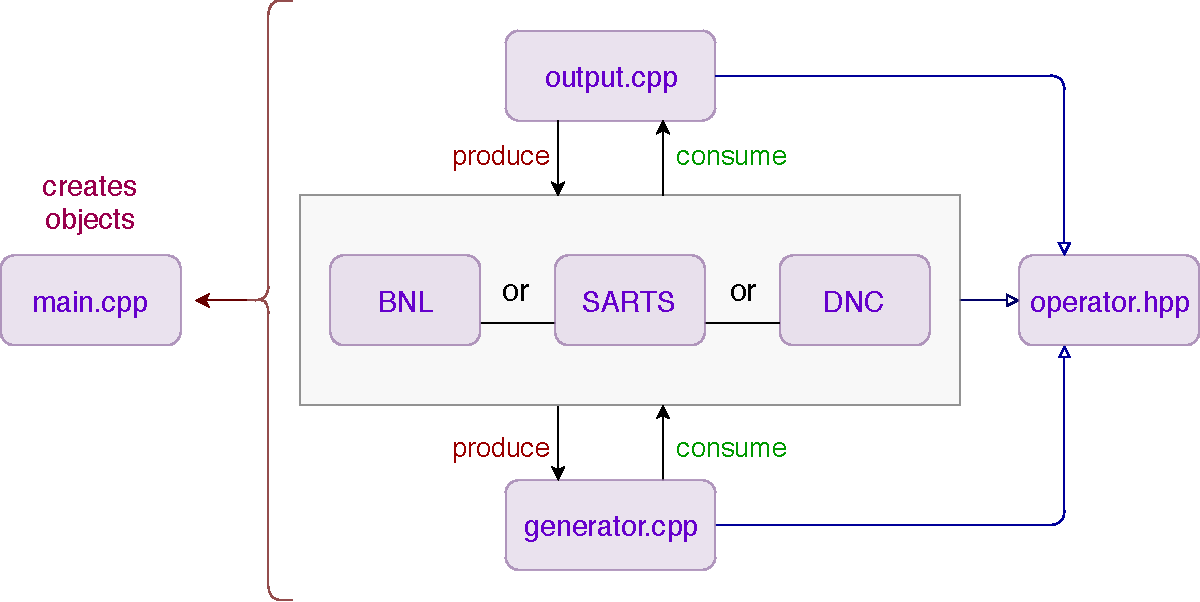
\includegraphics[width=0.9\linewidth]{figures/test-setup}
\caption{Test Setup with Sample Algorithms}
\label{fig:test-setup}
\end{figure}

While tree-based skyline algorithms, such as ST-S and SARTS, can only realistically work with categorical attributes, other general-purpose algorithms are not restricted to categorical attribute domains. Therefore, all tests that include the algorithms ST-S and SARTS were conducted using a limited set of integers as categories, ranging from 0 to 255. All other tests were performed with continuous attributes, represented as \textit{double} values. 

The memory usage of N-Tree and ART was captured with the tool Valgrind Massif. It is a heap profiler capable of determining how much heap memory the program is using at particular points in time. 

%\subsection{Measurement Metrics}
%The two metrics measured by performance tests were running time and main memory usage. For each of the running-time-entries within the test results, the median value from three independent test runs was taken, in order to reduce volatility of the results. 

%The two metrics measured by performance tests were running time and main memory usage. The running time was measured for all the algorithms in test, namely: BNL Volcano, BNL Produce/Consume, Naive Nested-Loops, parallel Naive Nested-Loops, DNC, parallel DNC, ST-S, parallel ST-S, SARTS and parallel SARTS. % adjust this list with respect to i/m and p/c
%The running time was captured in dependence of the number of tuples, the dimensionality of the input, as well as the number of threads that can be used in parallel. For each of the running-time-entries within the test results, the median value from three independent test runs was taken, in order to reduce volatility/variation of the results. 
%
%The main memory usage was measured for the N-Tree as well as for the ART tree, each in the scope of their respective algorithm ST-S or SARTS. 
%These measurements were conducted in dependence of the number of tuples and the dimensionality of the input. 
%
%While tree-based skyline algorithms, such as ST-S and SARTS, can only realistically work with categorical attributes, other general-purpose algorithms are not restricted to categorical attribute domains. Therefore, all tests that include the algorithms ST-S and SARTS were conducted using a limited set of integers as categories, ranging from 0 to 255. Other tests that do not include tree-based algorithms were performed with continuous attributes, represented as \textit{double} values in C++. 

%\subsection{Tools}
% Terminal Output
%When measuring the time taken to compute the skyline by each of the algorithms, the time point before the start of the algorithm and the time point after its finish were captured. The difference between the two points in time was interpreted as the running time of the particular algorithm. Any operations belonging to the environment of the algorithms, such as printing the output, generating the dataset, or freeing the memory after computation were \textit{not} included in their running time.  

% Valgrind Memcheck
%Before measuring the memory usage within ST-S and SARTS, it was made sure that no memory leaks exist in any of the two algorithms. This was done with the help of Valgrind Memcheck, which is a tool for memory error detection. 

% Valgrind Massif
%The main memory usage itself was captured with the tool Valgrind Massif. It is a heap profiler capable of determining how much heap memory the program is using at particular points in time. 
%This is done by making multiple snapshots of the heap's current state during runtime. In addition to that, at some points of program execution, which Massif considers especially relevant, it captures detailed snapshots, telling precisely which part of the code is responsible for which block of the allocated memory. 

\section{Results}
% expectations
%It is expected for the parallelized algorithms to outperform their sequential counterparts with a rising number of tuples and threads. In addition to that, the ART tree is supposed to show similar performance to the N-Tree in terms of running time, while having the advantage of lower space consumption. The two query pipelining models Volcano and produce/consume are expected to show mostly similar evaluation times. 
In the following, the results of the conducted measurements are presented. 

\subsection{Computation Time}
% Notes: 
% Bei jedem parallelisierten Algorithmus gibt es auch unparallelisierte Blöcke, die ganz normal skalieren. D.h. auch, dass die Performance nicht immer z.b. 4 x so gut ist wie nicht parallelisiert. z.b mutex, transport der tupel durch die pipeline, etc. 

\subsubsection{Volcano and Produce/Consume} \label{section:models-test-comparison}
To begin with, the two query pipelining approaches Volcano and produce/consume were compared to each other. For this purpose, two different variants of the Block-Nested-Loops algorithm were implemented. Both versions can be found in the Appendix \ref{appendix-code} to this work. 
% Bnl Volcano vs. Bnl produce/consume
\begin{figure}[h]
	\centering
	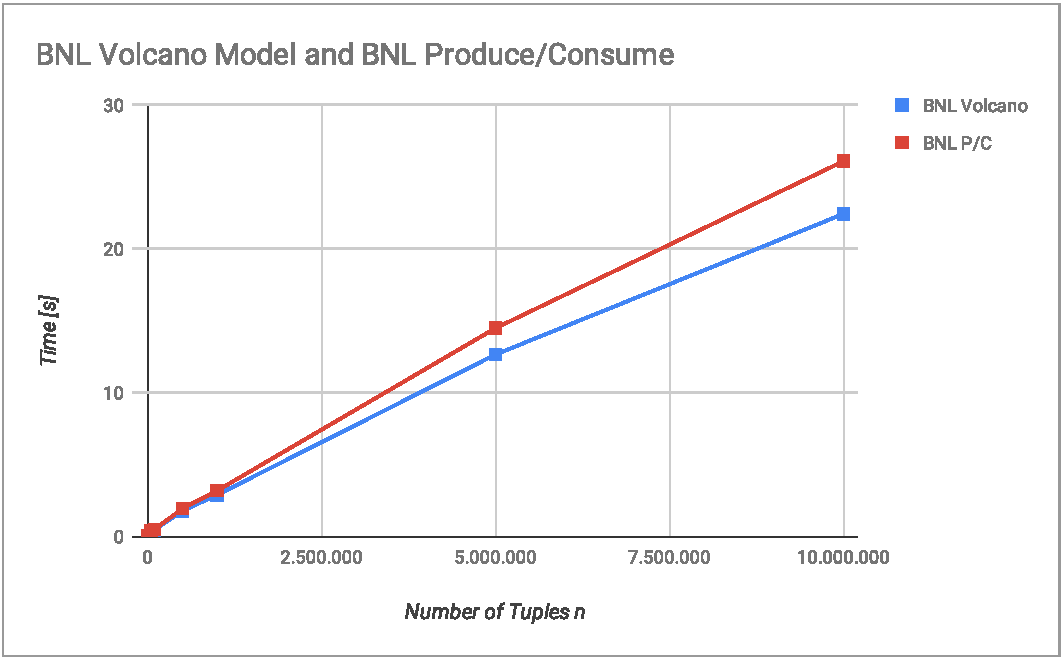
\includegraphics[width=1\linewidth]{figures/im-vs-pc}
	\caption{Comparison of Volcano Model and Produce/Consume Concept by Running Time}
	\label{fig:im-vs-pc}
\end{figure}
The results of the comparison (Fig.~\ref{fig:im-vs-pc}) show that up to a threshold of about 1 million tuples the running time of both BNL Volcano and BNL p/c is virtually the same. With the number of tuples further rising, the Volcano version consistently outperforms the produce/consume version. Therefore, the conclusion can be drawn that while the performance of Volcano is only slightly better than that of produce/consume, Volcano model is still the way to go for query pipelining. However, one should keep in mind that the produce/consume concept used in this work is not the original one, which would also include code generation, as explained in section \ref{section:methods-frameworks}. 
The underlying numbers to this comparison are given in form of a table in Appendix \ref{appendix-performance}. 

\subsubsection{Non-Progressive Algorithms}
Non-progressive skyline algorithms included in this work are Block-Nested-Loops and Divide-and-Conquer. In all three of the conducted tests, BNL proves that it scales significantly better than DNC. It shows overall better performance with rising numbers of tuples (Fig.~\ref{fig:non-progressive-n}), dimensions (Fig.~\ref{fig:non-progressive-dim}), and also threads (Fig.~\ref{fig:non-progressive-threads}). The same applies to the parallelized version of DNC. While it does perform better than the sequential version of DNC, it still cannot keep up with BNL in any of the tests. 

Herewith, the results are similar to the ones produced in the original paper \cite{kossmann}, where BNL and DNC were first introduced. In their evaluation, the authors showed that basic BNL significantly outperforms basic DNC for larger $n$. It is remarkable that the results measured within this work are significantly better than the results in \cite{kossmann} for both BNL and DNC. This is, however, not surprising, regarding the lack of I/O operations as well as a much more powerful testing machine this time. 

On the large scale of comparison between BNL and DNC, the two versions of BNL, namely Volcano style and Produce/Consume perform virtually the same in all three tests. There is, however, a slight difference between the two versions, as previously shown in this section. The concrete numbers measured within the tests can be found in Appendix \ref{appendix-performance}. 

% Non-Progressive Algorithms by n
\begin{figure}[h]
	\centering
	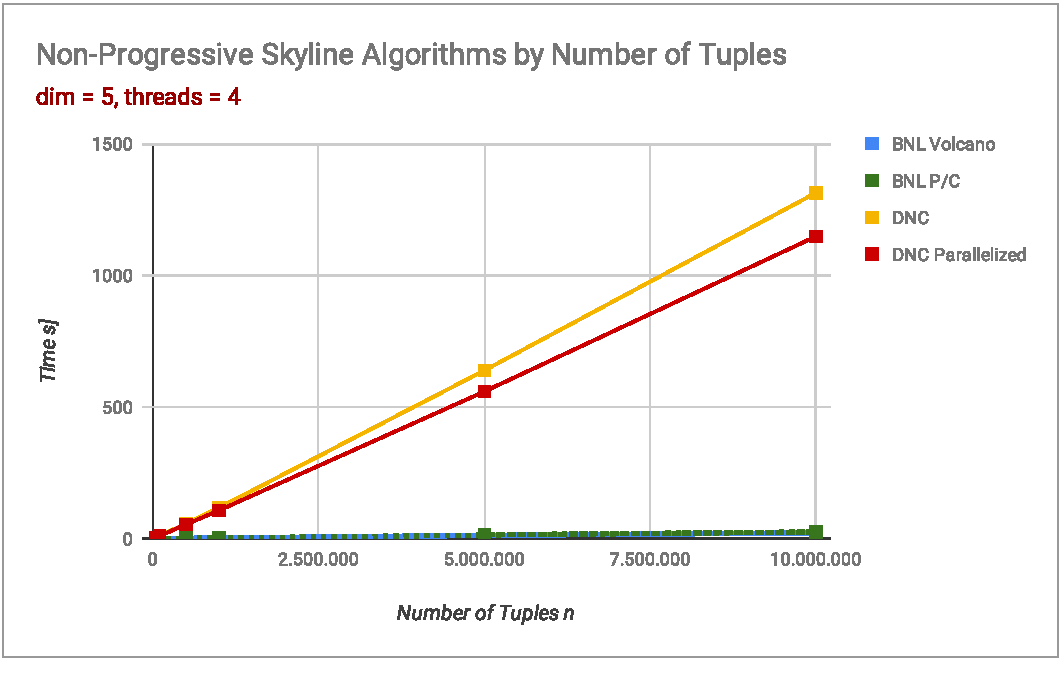
\includegraphics[width=1\linewidth]{figures/non-progressive-n}
	\caption{Running Time of Non-Progressive Algorithms by Number of Tuples}
	\label{fig:non-progressive-n}
\end{figure}

% Non-Progressive Algorithms by dim
\begin{figure}[H]
	\centering
	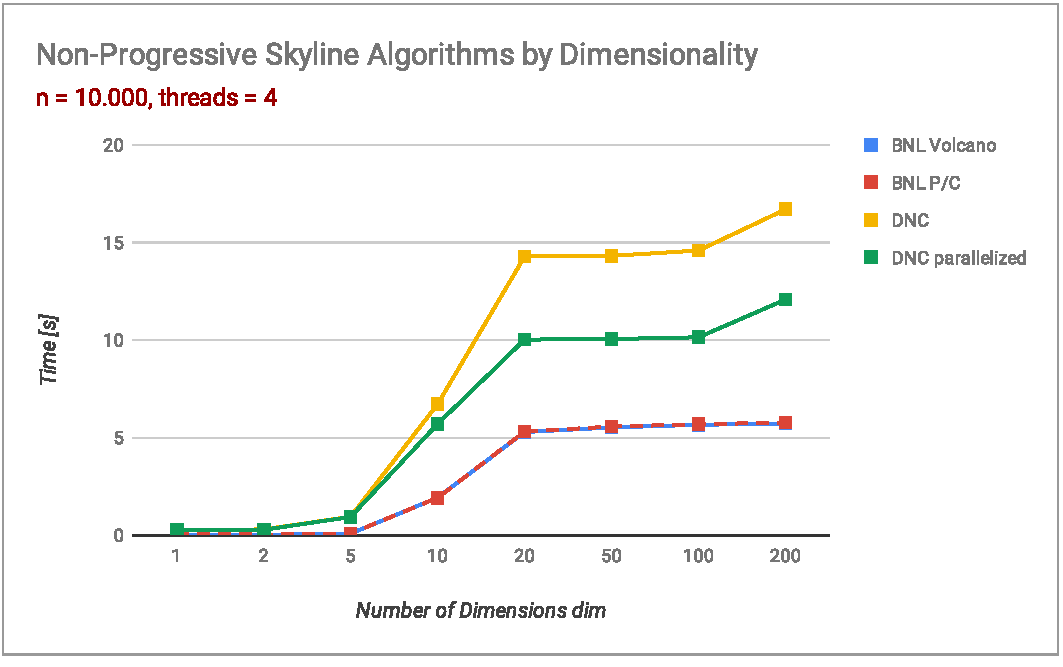
\includegraphics[width=1\linewidth]{figures/non-progressive-dim}
	\caption{Running Time of Non-Progressive Algorithms by Dimensionality}
	\label{fig:non-progressive-dim}
\end{figure}

% Non-Progressive Algorithms by threads
\begin{figure}[h]
	\centering
	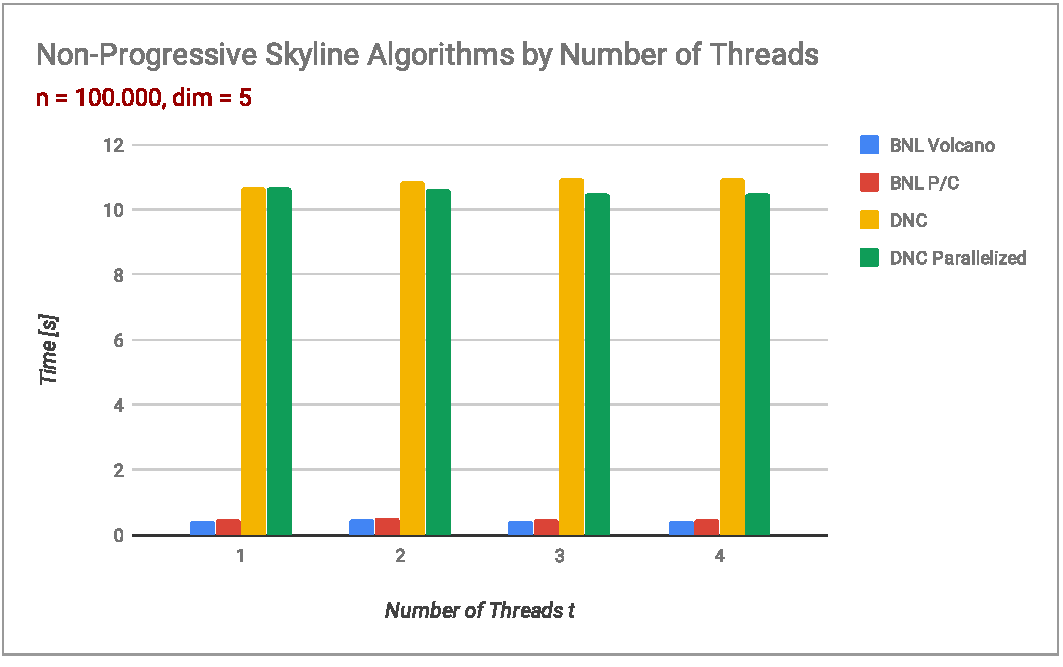
\includegraphics[width=1\linewidth]{figures/non-progressive-threads}
	\caption{Running Time of Non-Progressive Algorithms by Number of Threads}
	\label{fig:non-progressive-threads}
\end{figure}

\subsubsection{Progressive Algorithms}
Despite being the arguably simplest skyline algorithm to date, Naive-Nested-Loops can be both progressive and parallelizable if implemented correctly. This is what this work makes use of in order to make it comparable with the two newer algorithms ST-S and SARTS. 

As expected, for a rising number of tuples $n$ both ST-S and SARTS perform extremely well. As shown in Fig.~\ref{fig:progressive-n}, they significantly outperform Naive-Nested-Loops for both middle-range and large $n$. This is not surprising, considering that ST-S and SARTS were both specifically developed for large categorical datasets. It is due to the efficient tree structures used,  that dominance checks can be conducted very efficiently, and depend less on the number of tuples than on the dimensionality of the dataset (section \ref{section:art-characteristics}). 

% Progressive Algorithms by n
\begin{figure}[h]
	\centering
	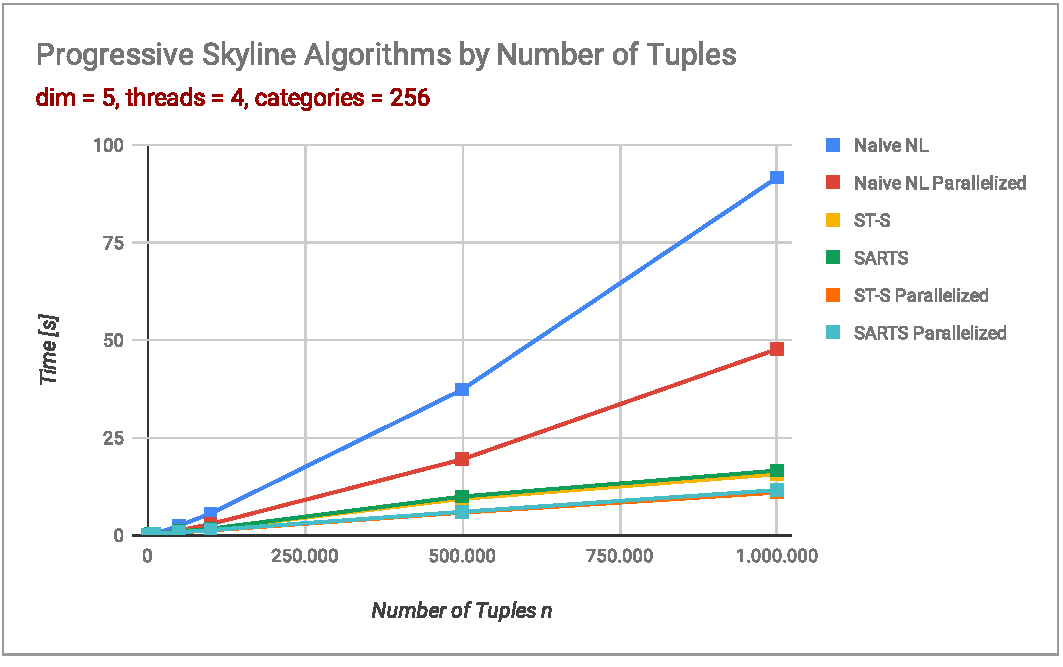
\includegraphics[width=1\linewidth]{figures/progressive-n}
	\caption{Running Time of Progressive Algorithms by Number of Tuples}
	\label{fig:progressive-n}
\end{figure}

A more close-up comparison of ST-S and SARTS is shown in Fig.~\ref{fig:progressive-n-2}. It can be seen that the parallelized versions of both algorithms start outperforming their sequential counterparts at a dataset size of about 100,000 tuples. While the ST-S and SARTS algorithms generally go ``hand-in-hand'' for both sequential and parallelized versions, the ST-S algorithm is slightly better than SARTS for large $n$. This advantage, however, seems of lesser significance in comparison to the memory usage gains of the SARTS algorithm, which will be presented in the next section of this work. 

% Progressive Algorithms by n - second
\begin{figure}[H]
	\centering
	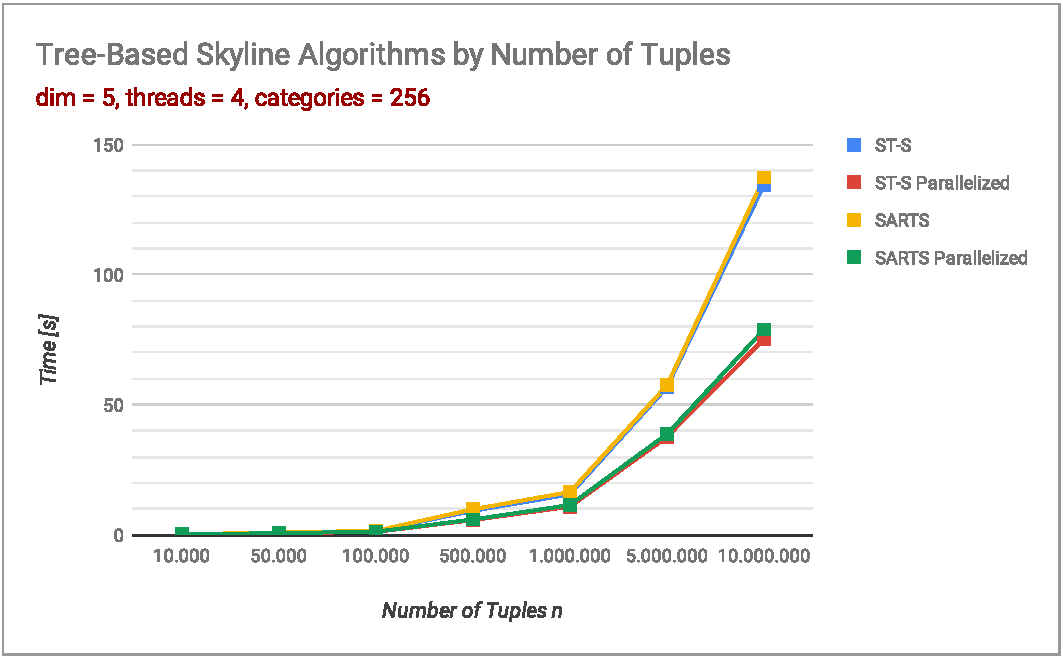
\includegraphics[width=1\linewidth]{figures/progressive-n-2}
	\caption{Running Time of Tree-Based Progressive Algorithms by Number of Tuples}
	\label{fig:progressive-n-2}
\end{figure}

When looking at the results of scaling with dimensionality, a somewhat different picture emerges (Fig.~\ref{fig:progressive-dim}). In this test, Naive-Nested-Loops significantly outperforms both parallelized and sequential versions of ST-S and SARTS. The reason for this is that radix-based tree structures --- which N-Tree and ART both are --- generally scale badly with longer keys. This is the trade-off they have to take for very efficient scaling with the number of elements inserted. The longer the keys of the dataset are, the higher the tree gets, and the longer it takes to traverse the tree from top to bottom. In the application area of skyline computation, the length of a key corresponds to the dimensionality of a tuple. Hence, the more dimensions the tuples of a dataset have, the less efficient tree-based dominance checks become. This is exactly what can be seen in Fig.~\ref{fig:progressive-dim}. 
It also explains why parallelized versions of the algorithms perform worse than the sequential ones. The parallelization of ST-S and SARTS is based on multiple sub-trees used to compute subset skylines before merging them into one final skyline. Thus, the sub-trees also underlie the ``curse of dimensionality''. 

% Progressive Algorithms by dim
\begin{figure}[h]
	\centering
	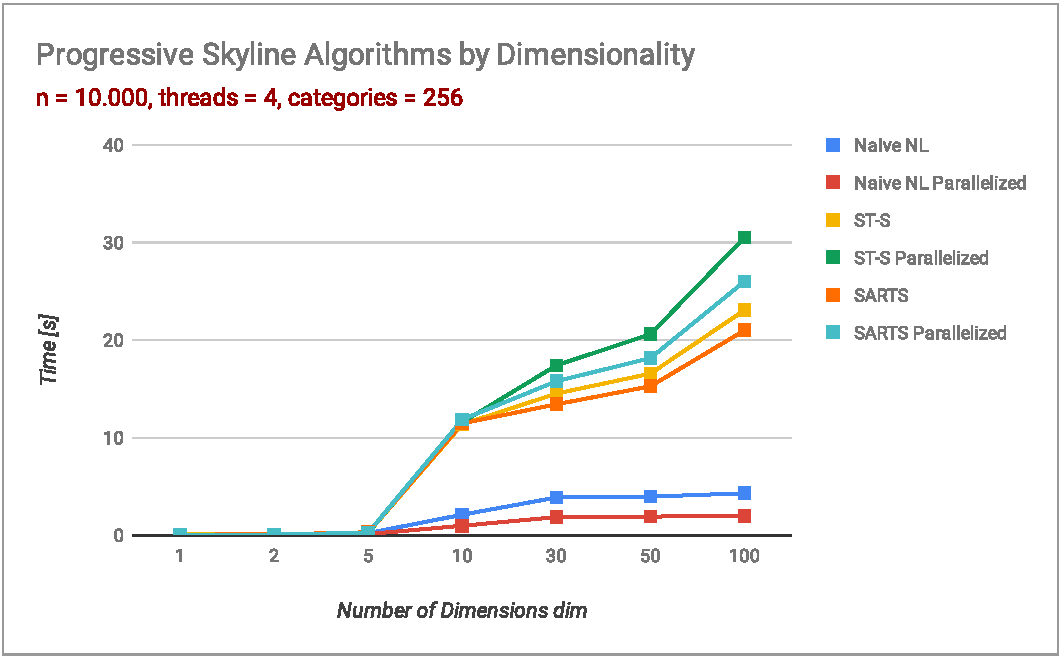
\includegraphics[width=1\linewidth]{figures/progressive-dim}
	\caption{Running Time of Progressive Algorithms by Dimensionality}
	\label{fig:progressive-dim}
\end{figure}

The comparison of progressive algorithms depending on the number of threads available shows that ST-S and SARTS outperform Naive-Nested-Loops for both parallelized and non-parallelized versions. As expected, the time consumption of the parallelized algorithms gets less with a rising number of threads. This means that the parallelization approaches taken in chapter \ref{chapter:Parallelization} produce the desirable performance improvements. While on 1 and 2 threads ST-S and SARTS are a bit faster in their sequential version, on 3 cores and more the parallelized versions show better performance. For the Naive-Nested-Loops algorithm this already happens from 2 threads and up. 
The slightly worse performance of tree-based algorithms on 1 and 2 threads is likely due to the additional overhead required to partition the original dataset, to create a sub-tree for each of the threads, as well as to set up the threads themselves. The performance improvements are expected to become more noticeable if the algorithms run on more than 4 threads, like for instance 8 or 16. 

% Progressive Algorithms by threads
\begin{figure}[h]
	\centering
	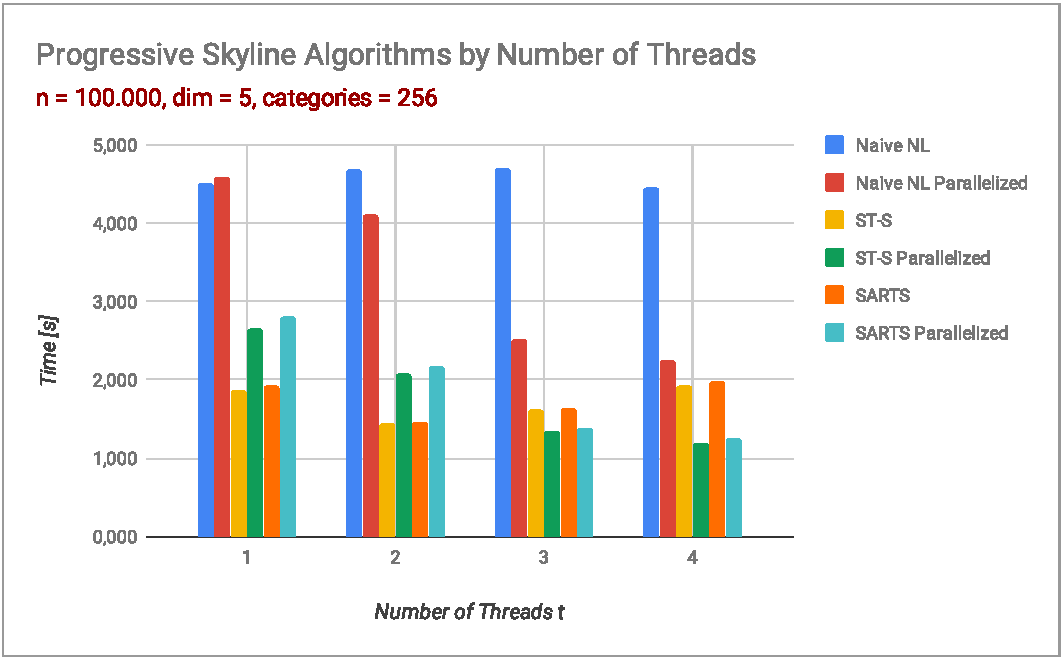
\includegraphics[width=1\linewidth]{figures/progressive-threads}
	\caption{Running Time of Progressive Algorithms by Number of Threads}
	\label{fig:progressive-threads}
\end{figure}

\subsection{Memory Usage}
Within the last two tests, the main memory usage of the ART tree was compared to that of the N-Tree. 
Fig.~\ref{fig:memory-usage-n} shows that the ART tree has significantly lower space consumption than the N-Tree for every $n$ in test. While for $n$ = 10 ART uses about 22-times less memory than N-Tree, even for large $n$, such as $10^{6}$, it still uses appx. 20-times less space than N-Tree. The measured numbers can be found in Appendix \ref{appendix-performance} to this work. 

% memory usage by n
\begin{figure}[h]
	\centering
	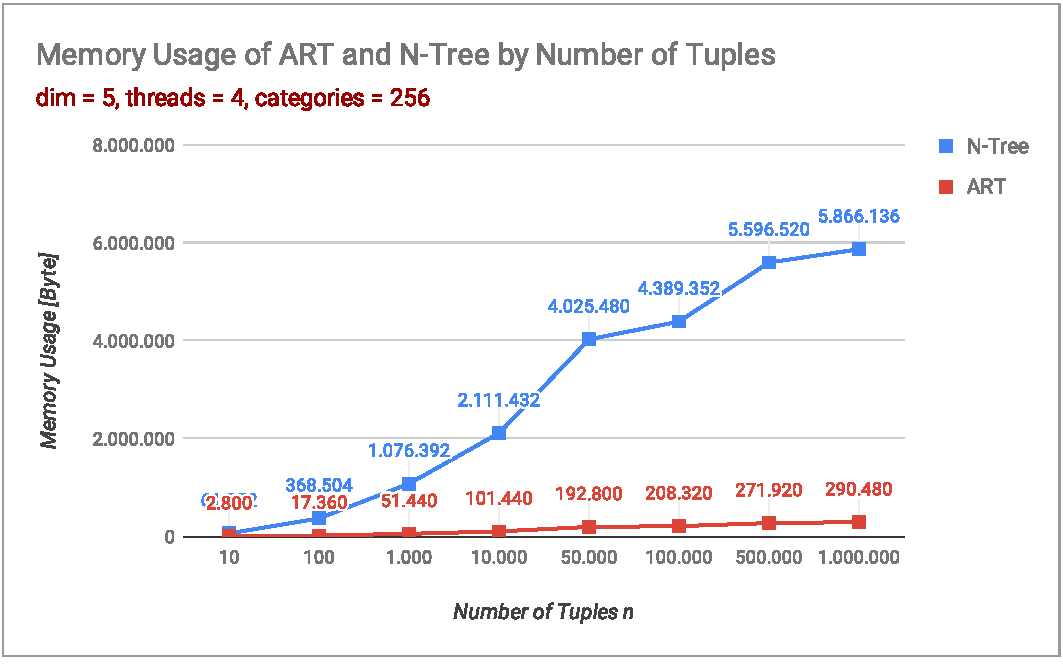
\includegraphics[width=1\linewidth]{figures/memory-usage-n}
	\caption{Memory Usage of ART and N-Tree by Number of Tuples}
	\label{fig:memory-usage-n}
\end{figure}

A similar picture can be seen when looking at memory consumption scaling with dimensionality in Fig.~\ref{fig:memory-usage-dim}. While for low numbers of $dim$, the ART tree already performs better than the N-Tree, it generally scales much more efficiently with high dimensionality. At the point of $dim$ = 50 the ART uses only around $\frac{1}{38}$ of the memory that N-Tree does. Thus, it can be concluded that the SARTS algorithm is significantly more memory-efficient than ST-S due to the usage of ART. 

% memory usage by dim
\begin{figure}[h]
	\centering
	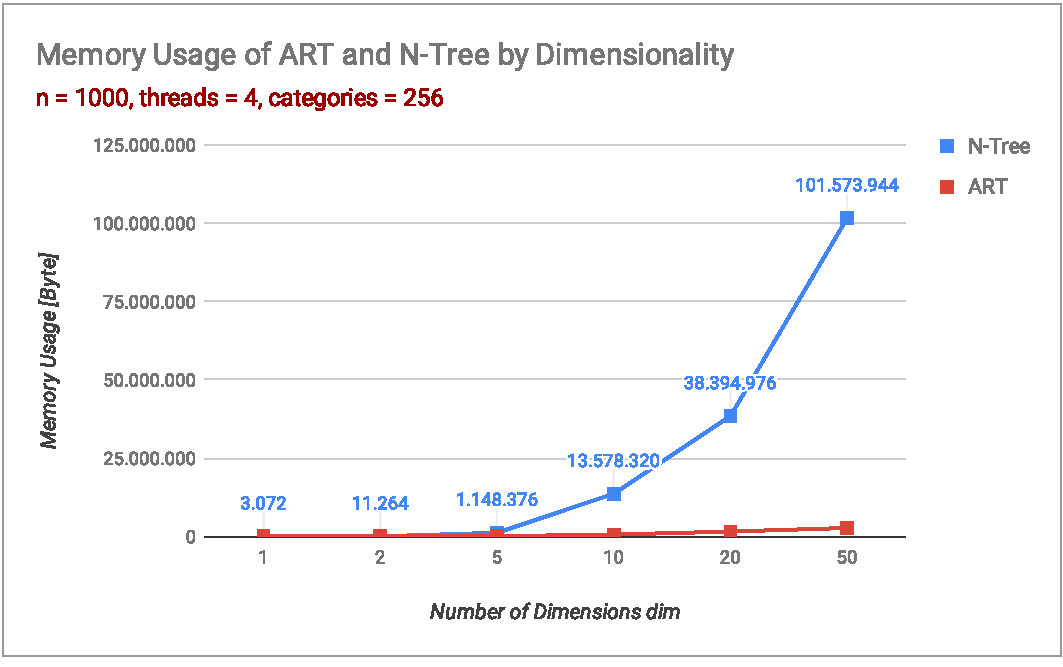
\includegraphics[width=1\linewidth]{figures/memory-usage-dim}
	\caption{Memory Usage of ART and N-Tree by Dimensionality}
	\label{fig:memory-usage-dim}
\end{figure}




		\chapter{Conclusion}
\label{chapter:Conclusion}

\section{Summary}
In this work, three of the basic skyline algorithms Naive-Nested-Loops, Block-Nested-Loops and Divide-and-Conquer, as well as the newer ST-S algorithm were introduced. The algorithms were placed into the ``big picture'' of the current state-of-the-art skyline algorithms and explained in detail. Thereafter, the novel skyline algorithm SARTS, which utilizes the highly efficient ART tree, was presented. The algorithm keeps all the advantages of ST-S, while being significantly more memory-efficient at the same time. The algorithms were parallelized using different approaches and frameworks, which were explained in greater detail. In the last chapter, an evaluation of the conducted tests was carried out and the outcomes analyzed. 

With the results of this work, the following points should be considered when choosing the right skyline algorithm for the particular use case: 
\begin{itemize}
	\item When the application scenario assumes continuous attribute values and does not require progressive behavior, then Block-Nested-Loops seems to be a very potent ``all-rounder'' algorithm, well suited for both I/O-intensive as well as in-memory databases. At this point, some of the newer algorithms based on Block-Nested-Loops should be considered, such as SFS~\cite{sfs} and SaLSa~\cite{salsa}. The presorting and the threshold approaches showed that they can improve an algorithm such as ST-S, and thus can be recommended to be applied to BNL as well. 
	\item In a scenario where progressiveness is important, an online-capable algorithm such as ST-S or SARTS should be chosen. Both algorithms perform excellently for medium-range to high $n$ and provide good scalability in parallelized environments. While tree-based algorithms do not scale well with high dimensionality, most online services seem to have a high number of database entries with mostly low dimensionality nowadays\footnote{Consider a database holding around 1 million hotels with 5-10 different categorical attributes each for this purpose.}.
	\item In environments that require efficient memory usage SARTS is highly recommended to be chosen over ST-S due to its significantly lower space consumption. 
\end{itemize}

\section{Outlook}
% parallelization
While the parallelization approaches introduced in this work showed to improve the respective sequential versions of the algorithms, some of them have the potential to perform even better when running on more than 4 threads. This could be further tested, provided that a suiting machine is available. 

% Art baum mit path compression und lazy expansion
The current version of the SARTS algorithm already keeps up with ST-S in terms of computation time, and overtakes it by far in terms of efficient memory usage. Nevertheless, it still can be improved by utilizing not the basic, but the full version of the ART tree, including both lazy expansion and path compression. These techniques enable faster insert operations and dominance checks, and also save even more memory by leaving out unnecessary nodes. It is expected that with these improvements the SARTS algorithm would bypass ST-S both in speed and in efficiency of memory usage. The only (known) successor to ST-S to date is the algorithm TA-SKY, also proposed by the same authors in \cite{rahman}. Thus, it would be interesting to compare an improved version of SARTS to TA-SKY in terms of time and memory management. 

% integration into a DBMS
SARTS was originally developed in the context of an in-memory database, such as HyPer~\cite{hyper}. Still, it also seems suitable for I/O-intensive DBMS due to BNL being one of its ``ancestors''. While performance tests in this work showed that SARTS can deal quite well with synthetic datasets, it is always sensible to test an algorithm on real-world datasets. For this reason, it can be recommended to integrate SARTS in a database system, in order to see how well it fares in this environment. 

% online algorithm
As SARTS should be primarily used as an online algorithm, it also appears sensible to test it within a database system which demands its algorithms to work progressively, i.e. to deliver first results before the entire skyline is computed. Some sort of interactive web application seems fit for this purpose. 
		
%		\part[The 2nd Part]{The Second Part}
%		\label{part:secondP}		
		
		% ---------------------------------------------------------------------------
		%
		% Appendix
		%
		% ---------------------------------------------------------------------------
		
		\part*{Appendix}
		\addcontentsline{toc}{part}{Appendix}
		
		\appendix %---------------------------------------
		
			\chapter{Datastream Extraction Tool Manual} \label{appendix-dset-manual}
\captionsetup{margin=10pt,font=large,labelfont=bf,textfont={bf}}

The full version of the Datastream Extraction Tool Manual can be found in the project folder of the Google Drive repository under \url{https://bit.ly/3rB3lqg}. 

\section{Introduction}
The Datastream Extraction Tool is an application that allows the user to download financial data from Thomson Reuters Datastream without the overhead of doing it manually in Excel. The tool was created specifically for large static and time-series requests, and supports long-duration downloads of data. 

\section{Installation}
Please, be aware of the following: 
\begin{itemize}
	\item The application can only be run on Windows computers. It cannot be ported to MacOS or Linux, as the Thomson Reuters Excel add-in is only available for Windows, and also because the VBA (Visual Basic for Applications) version on Unix-based computers is a different one than on Windows computers. 
	\item While the application can generally be run on remote computers as well, it can be rather inconvenient. On the one hand, remote computers tend to be less stable in terms of internet connection and add-in connectivity. And additionally, the remote computers of TUM-SOM have rather poor performance (especially disk access!), which would constrain the data download. Furthermore, remote computers automatically shut down after some time, which makes downloading large data loads problematic. For smaller requests though, that take up to 1 hour of download time, the remote execution should suffice. 
\end{itemize}

\subsection{Prerequisites}
Please make sure that the following environment is established before you proceed with the installation.
\begin{itemize}
	\item Make sure you have a valid \textbf{Microsoft Office Installation}. The application was tested with Office 365, but it should also run with other recent Office environments.
	\item Make sure that \textbf{Thomson Reuters Eikon \& Datastream} is installed. If you install it for the first time, please ensure that the Datastream add-on in the Excel plug-in is enabled. 
	\item Make sure that you have an up-to-date version of \textbf{Python 3} installed. Python 3 is different from Python 2; with Python 2 the application will not work. 
	\item Make sure that in Windows Power Options you select that your PC "never" goes to sleep. Since otherwise this can interrupt long-running downloads. 
\end{itemize}

\subsection{Download}
Follow these steps to install the application on your computer: 
\begin{enumerate}
	\item Download the \textit{Shippable} folder from \url{https://bit.ly/2VfT058} to your computer. Choose a location with enough free space, as the downloaded data will be stored in-place. 
	\item Unzip the downloaded file. You can rename the root folder from \textit{Shippable} to a different name at your convenience. Please, do \textbf{not} rename any of the folders or files inside. Such changes would need to be propagated to the program code. 
	\item In the \textit{Shippable }folder, you will find a file called \textbf{\textit{prerequisites.py}}. You need to run this file with Python. You can do so by e.g. right-clicking on the file, selecting "Open with" and then choosing Python. It will then automatically install external Python packages needed for the app. 
\end{enumerate}

\subsection{Settings}
Finally, you will need to adjust some settings in Excel the first time you install the application. For this purpose, open the file called \textit{RequestTable.xlsm} in the \textit{Shippabl}e folder. 

The first time you open it, you might get prompted to activate file contents or to allow modifications, etc. Please agree to all such messages. 

Further, take care of the following settings: 
\begin{itemize}
	\item Make sure that both the \textit{Thomson Reuters} tab and the \textit{Thomson Reuters Datastream} tab show in the tab panel of the Excel document. 
	\item In the Thomson Reuters tab go to Settings $=>$ Sign-In $=>$ choose to automatically sign-in whenever Office is started. 
	\item Go to File $ => $ Options $ => $ Trust Center $ => $ Trust Center Settings and do: 
	\begin{itemize}
		\item Macro Settings $ => $ select "\textit{Enable all macros}" and check "\textit{Trust access to the VBA project object model}". 
		\item Protected View $ => $ uncheck all boxes except for "\textit{Outlook attachments}". 
		\item Add-ins $ => $ uncheck all boxes.
		\item External Content $ => $ select "\textit{Enable all Data Connections}", "\textit{Enable automatic update for all Workbook Links}", "\textit{Enable all Linked Data Types}".
	\end{itemize}
	\item Go to File $ => $ Options $ =>  $Customize Ribbon $ => $ select \textit{Main Tabs} on the right $ => $ check the \textit{Developer, Add-ins, Thomson Reuters}, and \textit{Thomson Reuters Datastream} tabs. 
	\item Go to File $ => $ Options $ => $ Advanced $ => $ section \textit{General} $ => $ uncheck option \textit{Ask to update automatic links}. 
	\item Go to File $ => $ Options $ => $ Add-ins and make sure that the add-in \textit{Thomson Reuters Eikon - Microsoft Office }is listed among \textit{Active Application Add-ins}. It should be. If not, refer to the Troubleshooting section. 
	\item Press "Alt + F11" (the VBA editor will appear) $ => $ go to Tools $ => $ References $ => $ check the box near "\textit{Microsoft Scripting Runtime}"
\end{itemize}

Now, you should be well set to run the application.

\section{Usage}
You can start the Datastream Extraction Tool by running the file \textbf{\textit{ds\_extraction\_tool.py}} with Python. 

If you encounter a problem, some other prerequisites on your computer might be missing that might not have been covered in this guide. In that case, please contact the project developer. 


\chapter{C++ Code} \label{appendix-code}
\usemintedstyle{bw}

\section{Dominates Operation for NNL, BNL and DNC}
\begin{minted}[tabsize=3,breaklines,fontsize=\small]{c++}
/**
* Checks whether one tuple dominates the other and returns true|false
* @param dominator the tuple to check for dominating
* @param dominated the tuple to check for being dominated
*/
bool dominates(const std::vector<int> &dominator, const std::vector<int> &dominated){
	bool flag = true;
	for(std::vector<int>::size_type i = 0; i< dominated.size(); i++){
		if(dominator[i] > dominated[i]) return false;
		if(dominated[i] > dominator[i]) flag = false;
	}
	if(flag) return false;
	return true;
}
\end{minted}

\section{Naive-Nested-Loops}
\begin{minted}[tabsize=3,breaklines,fontsize=\small]{c++}
void computeSkylineProduce(){
	for(std::size_t i = 0; i < storage.size(); i++){
		bool not_dominated = true;
		for(std::size_t j = 0; j < storage.size(); j++){
			if(i != j){
				if(dominates(storage[j], storage[i])){
					not_dominated = false;
					break;
				}
			}
		}
		if(not_dominated){
			parent->consume(storage[i]);
		}
	}
}
\end{minted}

\section{Naive-Nested-Loops Parallelized}
\begin{minted}[tabsize=3,breaklines,fontsize=\small]{c++}
void computeSkylineProduceParallel(){
	const std::vector<std::vector<int>> storage = this->storage;
	CatOperator *parent = this->parent;
	parallel_for(std::size_t(0), storage.size(), [this, storage, parent]( std::size_t i ) {
		bool not_dominated = true;
		bool flag = false;
		for(std::size_t j = 0; j < storage.size() && !flag; j++){
			if(i != j){
				if(dominates(storage[j], storage[i])){
					not_dominated = false;
					flag = true;
				}
			}
		}
		// The following mutex slows down the parallelization, but provides an easy way to avoid race conditions
		// In case no mutex is used, the programmer needs to make sure that no race condition occurs in the following if-block
		static spin_mutex mtx;
		spin_mutex::scoped_lock lock(mtx);
		if(not_dominated){
			parent->consume(storage[i]);
		}
	} );
}
\end{minted}

\section{Block-Nested-Loops Volcano Model}
\begin{minted}[tabsize=3,breaklines,fontsize=\small]{c++}
void computeSkyline(){
	// storage is the window here
	storage.push_back(child->getNext());
	while(true){
		std::vector<int> tuple = child->getNext();
		if(!tuple.empty()){
			storage.push_back(tuple);
			for(std::size_t j = 0; j < storage.size()-1; j++){
				if(dominates(storage.back(), storage[j])){
					storage.erase(storage.begin() + j);
					j--;
				}
				else if (dominates(storage[j], storage.back())){
					storage.erase(storage.begin() + storage.size()-1);
					break;
				}
			}
		}
		else break;
	}
}
\end{minted}

\section{Block-Nested-Loops Produce/Consume}
\begin{minted}[tabsize=3,breaklines,fontsize=\small]{c++}
void computeSkylineProduce(){
	// storage contains tuples produced by the generator
	std::vector<std::vector<int>> window;
	window.push_back(storage[0]);
	for(std::size_t i = 1; i < storage.size(); i++){
		std::vector<int> tuple = storage[i];
		window.push_back(tuple);
		for(std::size_t j = 0; j < window.size()-1; j++){
			if(dominates(window.back(), window[j])){
				window.erase(window.begin() + j);
				j--;
			}
			else if (dominates(window[j], window.back())){
				window.erase(window.begin() + window.size()-1);
				break;
			}
		}
	}
	for(std::size_t i = 0; i < window.size(); i++){
		parent->consume(window[i]);
	}
}
\end{minted}

\section{Divide-and-Conquer}

\subsubsection{{\large Algorithm}}
\begin{minted}[tabsize=3,breaklines,fontsize=\small]{c++}
std::vector<std::vector<double>> computeSkyline(const std::vector<std::vector<double>> &M, const int &dimension){
	if(M.size() == 1) return M;
	
	std::vector<double> pivot = median(M, dimension-1); // dimension-1 because we need the last index
	std::pair<std::vector<std::vector<double>>, std::vector<std::vector<double>>> P = partition(M, dimension-1, pivot);
	
	std::vector<std::vector<double>> S_1, S_2;
	S_1 = computeSkyline(P.first, dimension);
	S_2 = computeSkyline(P.second, dimension);
	
	std::vector<std::vector<double>> result;
	std::vector<std::vector<double>> merge_result = mergeBasic(S_1, S_2, dimension);
	
	// Union S_1 and merge_result
	for(std::vector<std::vector<double>>::size_type i = 0; i < S_1.size(); i++){
		result.push_back(S_1[i]);
	}
	for(std::vector<std::vector<double>>::size_type i = 0; i < merge_result.size(); i++){
		result.push_back(merge_result[i]);
	}
	
	return result;
}
\end{minted}

\subsubsection{{\large Partition Operation}}
\begin{minted}[tabsize=3,breaklines,fontsize=\small]{c++}
std::pair<std::vector<std::vector<double>>, std::vector<std::vector<double>>> partition(const std::vector<std::vector<double>> &tuples, const int &dimension, const std::vector<double> &pivot){
	std::vector<std::vector<double>> P_1, P_2;
	std::pair<std::vector<std::vector<double>>, std::vector<std::vector<double>>> partitions;
	
	for(std::vector<std::vector<double>>::size_type i = 0; i < tuples.size(); i++){
		if(tuples[i][dimension] < pivot[dimension])
			P_1.push_back(tuples[i]);
		else
			P_2.push_back(tuples[i]);
	}
	
	partitions.first = P_1;
	partitions.second = P_2;
	
	return partitions;
}
\end{minted}
\subsubsection{{\large Merge Operation}}
\begin{minted}[tabsize=3,breaklines,fontsize=\small]{c++}
std::vector<std::vector<double>> mergeBasic(std::vector<std::vector<double>> S_1, const std::vector<std::vector<double>> &S_2, const int &dimension){
	std::vector<std::vector<double>> result;
	
	if(S_2.size() == 0) return result;
	
	if(S_1.size() == 1){ // trivial case - S_1 has only 1 tuple
		for(std::vector<std::vector<double>>::size_type i = 0; i < S_2.size(); i++){
			if(!dominates(S_1[0], S_2[i]))
				result.push_back(S_2[i]);
		}
	}
	else if(S_2.size() == 1){ // trivial case - S_2 has only 1 tuple
		result.push_back(S_2[0]);
		for(std::vector<std::vector<double>>::size_type i = 0; i < S_1.size(); i++){
			if(dominates(S_1[i], S_2[0])){
				result.erase(result.begin());
				break;
			}
		}
	}
	else if(S_1[0].size() == 2){ // low dimension
		// Min from S_1 according to dimension 1
		std::sort(S_1.begin(), S_1.end(), [](const std::vector<double> &a, const std::vector<double> &b){
			return a[0] < b[0];
		});
		std::vector<double> min = S_1[0];
		// Compare S_2 to Min according to dimension 1; in dimension 2 S_1 is always better
		for(std::vector<std::vector<double>>::size_type i = 0; i < S_2.size(); i++){
			if(S_2[i][0] < min[0]) result.push_back(S_2[i]);
		}
	}
	else{ // general case
		std::vector<double> pivot = median(S_1, dimension-1-1);
		std::pair<std::vector<std::vector<double>>, std::vector<std::vector<double>>> partitions_dim_1 = partition(S_1, dimension-1-1, pivot);
		std::pair<std::vector<std::vector<double>>, std::vector<std::vector<double>>> partitions_dim_2 = partition(S_2, dimension-1-1, pivot);
		std::vector<std::vector<double>> result_1, result_2, result_3;
		
		result_1 = mergeBasic(partitions_dim_1.first, partitions_dim_2.first, dimension);
		result_2 = mergeBasic(partitions_dim_1.second, partitions_dim_2.second, dimension);
		result_3 = mergeBasic(partitions_dim_1.first, result_2, dimension-1);
		
		// Union result_1 and result_3
		for(std::vector<std::vector<double>>::size_type i = 0; i < result_1.size(); i++){
			result.push_back(result_1[i]);
		}
		for(std::vector<std::vector<double>>::size_type i = 0; i < result_3.size(); i++){
			result.push_back(result_3[i]);
		}
	}
	
	return result;
}
\end{minted}

\section{ST-S/ SARTS}
\begin{minted}[tabsize=3,breaklines,fontsize=\small]{c++}
void computeSkylineProduce(){
	// pre-sort tuples in place
	sort(storage);
	std::vector<int> t_stop = storage[0];
	tree.insert(storage[0], tree.root, 0);
	parent->consume(storage[0]);
	for(std::size_t i = 1; i < storage.size(); i++){
		// stop if all the tuples left are dominated à-priori
		if((max(t_stop) <= min(storage[i])) && (t_stop != storage[i])){
			return;
		}
		// check for dominance
		if(!tree.is_dominated(storage[i], tree.root, 0, tree.score(storage[i]))){
			parent->consume(storage[i]);
			tree.insert(storage[i], tree.root, 0);
			if(max(storage[i]) < max(t_stop)){
				t_stop = storage[i];
			}
		}
	}
}
\end{minted}

\section{ST-S/ SARTS Parallelized}

\subsubsection{{\large Algorithm}}
\begin{minted}[tabsize=3,breaklines,fontsize=\small]{c++}
void computeSkylineProduce(){
	const std::vector<std::vector<int>> storage = this->storage;
	const std::size_t number_of_threads = NUMBER_OF_THREADS;
	std::vector<Tree*> subtrees;
	for(std::size_t i = 0; i < NUMBER_OF_THREADS; i++){
		Tree* subtree = new Tree(tree.get_attributes());
		subtrees.push_back(subtree);
	}
	std::future<void> futures[NUMBER_OF_THREADS];	
	// compute subquery skylines
	for(std::size_t i = 0; i < number_of_threads; i++){
		std::vector<std::vector<int>> subset;
		if(i == number_of_threads-1){
			subset.resize(storage.size() / number_of_threads + storage.size() % number_of_threads);
		}
		else{
			subset.resize(storage.size() / number_of_threads);
		}
		for(std::size_t j = 0; j < subset.size(); j++){
			subset[j] = storage[i*(storage.size()/number_of_threads) + j];
		}
		// Replace &ParallelSTS by &ParallelSARTS to receive SARTS
		futures[i] = std::async(std::launch::async, &ParallelSTS::computeSkylineSubset, this, i, subset, subtrees[i]);
	}
	for(std::size_t i = 0; i < NUMBER_OF_THREADS; i++){
		futures[i].get();
	}	
	// compute final skyline
	std::vector<std::vector<int>> input;
	for(std::size_t i = 0; i < subset_results.size(); i++){
		if(!subset_results[i].empty()){
			input.push_back(subset_results[i]);
		}
	}
	sort(input);
	std::vector<int> t_stop = input[0];
	tree.insert(input[0], tree.root, 0);
	parent->consume(input[0]);
	for(std::size_t i = 1; i < input.size(); i++){
		if((max(t_stop) <= min(input[i])) && (t_stop != input[i])){
			return;
		}
		if(!ntree.is_dominated(input[i], tree.root, 0, tree.score(input[i]))){
			parent->consume(input[i]);
			tree.insert(input[i], tree.root, 0);
			if(max(input[i]) < max(t_stop)){
				t_stop = input[i];
			}
		}
	}
	// free memory
	for(std::size_t i = 0; i < subtrees.size(); i++){
		if(subtrees[i] != nullptr) delete subtrees[i];
	}
}
\end{minted}
\subsubsection{{\large ComputeSkylineSubset Operation}}
\begin{minted}[tabsize=3,breaklines,fontsize=\small]{c++}
void computeSkylineSubset(unsigned threadNumber, std::vector<std::vector<int>> tuples, Tree* tree){
	// pre-sort tuples in place
	sort(tuples);
	std::vector<int> t_stop = tuples[0];
	tree->insert(tuples[0], tree->root, 0);
	subset_results[threadNumber * (subset_results.size() / NUMBER_OF_THREADS) + 0] = tuples[0];
	for(std::size_t k = 1; k < tuples.size(); k++){
		// stop if all tuples left are dominated a-priori
		if((max(t_stop) <= min(tuples[k])) && (t_stop != tuples[k])){
			return;
		}
		// check for dominance
		if(!tree->is_dominated(tuples[k], tree->root, 0, tree->score(tuples[k]))){
			subset_results[threadNumber * (subset_results.size() / NUMBER_OF_THREADS) + k] = tuples[k];
			tree->insert(tuples[k], tree->root, 0);
			if(max(tuples[k]) < max(t_stop)){
				t_stop = tuples[k];
			}
		}
	}
}
\end{minted}

\section{N-Tree}

\subsubsection{{\large Insert Operation}}
\begin{minted}[tabsize=3,breaklines,fontsize=\small]{c++}
void NTree::insert(const std::vector<int> &tuple, node* p, unsigned int level){
	if(level == 0){
		p->minScore = 0;
		p->maxScore = 0;
		for(std::size_t i = 0; i < tuple.size(); i++){
			p->maxScore += (int) (pow(2.0, (double) (tuple.size()-i)) * attributes[attributes.size()-1]);
		}
	}
	else{
		p->minScore = 0;
		for(std::size_t i = 0; i < level; i++){
			p->minScore += (int) (pow(2.0, (double) (tuple.size()-i)) * tuple[i]);
		}
		p->maxScore = p->minScore;
		for(std::size_t i = level; i < tuple.size(); i++){
			p->maxScore += (int) (pow(2.0, (double) (tuple.size()-i)) * attributes[attributes.size()-1]);
		}
	}
	if(level == tuple.size()){
		p->tupleIDs.push_back(tupleID++);
	}
	else{
		if(p->children.empty()){
			p->children.resize(attributes.size());
		}
		if(!p->children[tuple[level]]){
			p->children[tuple[level]]=new node();
		}
		insert(tuple, p->children[tuple[level]], level+1);
	}
}
\end{minted}

\subsubsection{{\large Is\_Dominated Operation}}
\begin{minted}[tabsize=3,breaklines,fontsize=\small]{c++}
bool NTree::is_dominated(const std::vector<int> &tuple, node* p, unsigned int level, unsigned int currentScore){
	if(p==nullptr || (currentScore < p->minScore)){
		return false;
	}
	if((level == tuple.size()) && (score(tuple) != p->minScore)){
		return true;
	}
	if((level == tuple.size()) && (score(tuple) == p->minScore)){
		return false;
	}
	// search the subtrees from left to right
	unsigned int weight = (int) (pow(2.0, (double) (tuple.size()-level)) * tuple[level]);
	for(int i = 0; i < tuple[level]; i++){
		if(is_dominated(tuple, p->children[i], level+1, currentScore + weight)){
			return true;
		}
	}
	if(is_dominated(tuple, p->children[tuple[level]], level+1, currentScore)){
		return true;
	}
	return false;
}
\end{minted}

\section{ART}
%\subsection{Nodes}

\subsubsection{{\large Insert Operation}}
\begin{minted}[tabsize=3,breaklines,fontsize=\small]{c++}
void ART::insert(const std::vector<int> &tuple, Node *&parent, Node *&current, unsigned int level){
	if(level == 0){
		current->minScore = 0;
		current->maxScore = 0;
		for(std::size_t i = 0; i < tuple.size(); i++){
			current->maxScore += (int) (pow(2.0, (double) (tuple.size()-i)) * attributes[attributes.size()-1]);
		}
	}
	else{
		current->minScore = 0;
		for(std::size_t i = 0; i < level; i++){
			current->minScore += (int) (pow(2.0, (double) (tuple.size()-i)) * tuple[i]);
		}
		current->maxScore = current->minScore;
		for(std::size_t i = level; i < tuple.size(); i++){
			current->maxScore += (int) (pow(2.0, (double) (tuple.size()-i)) * attributes[attributes.size()-1]);
		}
	}
	if(level == tuple.size()){
		current->tupleIDs.push_back(tupleID++);
	}
	else{
		Node* child = findChild(current, tuple[level]);
		if(!child){
			switch(current->type){
				case NodeType4:
					if(current->count == 4) 
						grow(parent, current, tuple[level-1]);
					break;
				case NodeType16:
					if(current->count == 16) 
						grow(parent, current, tuple[level-1]);
					break;
				case NodeType48:
					if(current->count == 48) 
						grow(parent, current, tuple[level-1]);
					break;
				case NodeType256:
				default:
					break;
			}
			child = newChild(current, tuple[level]);
		}
		insert(tuple, current, child, level+1);
	}
}
\end{minted}

\subsubsection{{\large Is\_Dominated Operation}}
\begin{minted}[tabsize=3,breaklines,fontsize=\small]{c++}
bool ART::is_dominated(const std::vector<int> &tuple, Node* p, unsigned int level, unsigned int currentScore){
	if(p==NULL || (currentScore < p->minScore)){
		return false;
	}
	if((level == tuple.size()) && (score(tuple) != p->minScore)){
		return true;
	}
	if((level == tuple.size()) && (score(tuple) == p->minScore)){
		return false;
	}
	// search the subtrees from left to right
	unsigned int weight = (int) (pow(2.0, (double) (tuple.size()-level)) * tuple[level]);
	for(int i = 0; i < tuple[level]; i++){
		Node* child = findChild(p, i);
		if(child){ // if child not null
			if(is_dominated(tuple, child, level+1, currentScore + weight)){
				return true;
			}
		}
	}
	Node* child = findChild(p, tuple[level]);
	if(child){
		if(is_dominated(tuple, child, level+1, currentScore)){
			return true;
		}
	}
	return false;
}
\end{minted}

\subsubsection{{\large Find\_Child Operation}}
\begin{minted}[tabsize=3,breaklines,fontsize=\small]{c++}
Node* ART::findChild(Node* parent, const int &attribute){
	switch(parent->type){
		case NodeType4: {
			Node4* node = static_cast<Node4*>(parent);
			for (unsigned i = 0; i < node->count; i++){
				if (node->key[i] == attribute){
					return node->children[i];
				}
			}
			return NULL;
		}
		case NodeType16: {
			Node16* node = static_cast<Node16*>(parent);
			for (unsigned i = 0; i < node->count; i++){
				if (node->key[i] == attribute){
					return node->children[i];
				}
			}
			return NULL;
		}
		case NodeType48: {
			Node48* node = static_cast<Node48*>(parent);
			if (node->childIndex[attribute] != emptyMarker){
				return node->children[node->childIndex[attribute]];
			}
			else
				return NULL;
		}
		case NodeType256: {
			Node256* node = static_cast<Node256*>(parent);
			return node->children[attribute];
		}
		default: {
			return NULL;
		}
	}
}
\end{minted}

\subsubsection{{\large New\_Child Operation}}
\begin{minted}[tabsize=3,breaklines,fontsize=\small]{c++}
Node* ART::newChild(Node *&node, const int &attribute){
	Node4* child = new Node4();
	switch(node->type){
		case NodeType4: {
			Node4* parent = static_cast<Node4*>(node);
			unsigned pos;
			// make free space for the new child entry
			for (pos = 0; (pos < parent->count) && (parent->key[pos] < attribute); pos++);
			memmove(parent->key+pos+1, parent->key+pos, parent->count-pos);
			memmove(parent->children+pos+1, parent->children+pos, (parent->count-pos)*sizeof(Node*));
			parent->key[pos] = attribute;
			parent->children[pos] = child;
			parent->count++;
			break;
		}
		case NodeType16: {
			Node16* parent = static_cast<Node16*>(node);
			unsigned pos;
			// make free space for the new child entry
			for (pos = 0; (pos < parent->count) && (parent->key[pos] < attribute); pos++);
			memmove(parent->key+pos+1, parent->key+pos, parent->count-pos);
			memmove(parent->children+pos+1, parent->children+pos, (parent->count-pos)*sizeof(Node*));
			parent->key[pos] = attribute;
			parent->children[pos] = child;
			parent->count++;
			break;
		}
		case NodeType48: {
			Node48* parent = static_cast<Node48*>(node);
			unsigned pos = parent->count;
			// if there are empty slots inbetween, use them instead of appending the child pointer at the end
			if(parent->children[pos]){
				for(pos = 0; parent->children[pos] != NULL; pos++);
			}
			parent->children[pos] = child;
			parent->childIndex[attribute] = pos;
			parent->count++;
			break;
		}
		case NodeType256: {
			Node256* parent = static_cast<Node256*>(node);
			parent->children[attribute] = child;
			parent->count++;
			break;
		}
		default:
			break;
	}
	return child;
}
\end{minted}

\subsubsection{{\large Grow Operation}}
\begin{minted}[tabsize=3,breaklines,fontsize=\small]{c++}
void ART::grow(Node *&parent, Node *&node, const int &indexOfCurrent){
	Node* newNode;
	switch(node->type){
		case NodeType4:
			newNode = new Node16();
			newNode->count = 4;
			for(std::size_t i = 0; i < 4; i++){
				static_cast<Node16*>(newNode)->key[i] = static_cast<Node4*>(node)->key[i];
			}
			for(std::size_t i = 0; i < 4; i++){
				static_cast<Node16*>(newNode)->children[i] = static_cast<Node4*>(node)->children[i];
			}
			break;
		case NodeType16:
			newNode = new Node48();
			newNode->count = 16;
			for(std::size_t i = 0; i < 16; i++){
				static_cast<Node48*>(newNode)->children[i] = static_cast<Node16*>(node)->children[i];
			}
			for (unsigned i = 0; i < node->count; i++){
				static_cast<Node48*>(newNode)->childIndex [static_cast<Node16*>(node)->key[i]] = i;
			}
			break;
		case NodeType48:
			newNode = new Node256();
			newNode->count = 48;
			for (unsigned i = 0; i < 256; i++){
				if (static_cast<Node48*>(node)->childIndex[i] != 48){ // slot not empty
					static_cast<Node256*>(newNode)->children[i] = static_cast<Node48*>(node)->children [static_cast<Node48*>(node)->childIndex[i]];
				}
			}
			break;
		default:
			break;
	}
	newNode->minScore = node->minScore;
	newNode->maxScore = node->maxScore;
	for(std::size_t i = 0; i < node->tupleIDs.size(); i++){
		newNode->tupleIDs[i] = node->tupleIDs[i];
	}
	
	if(node != root){
		// Code to updateParent() is not given for space reasons. Contact the author if needed. 
		updateParent(parent, newNode, indexOfCurrent);
	}
	delete node;
	node = newNode;
}
\end{minted}







	


  \clearemptydoublepage
  
  \bibliography{bibliography/literature}
	
 
\end{document}

